% ============================================================
% Báo cáo bài tập lớn CO5159 — Thực trạng mua bán dữ liệu cá nhân qua vụ việc sàn taphoammo.net và giải pháp pháp lý
% Biên dịch: pdfLaTeX (giống template, dùng vntex) hoặc XeLaTeX.
% Nội dung từng chương nằm trong chuongN.tex; trang bìa trong trang_bia.tex;
% danh mục tham khảo trong tai_lieu_tham_khao.tex (trích dẫn bằng \cite{khóa}).
% ============================================================
\documentclass[a4paper,12pt]{article}
\usepackage{iftex}
\ifPDFTeX
  \usepackage[T5]{fontenc}
  \usepackage[utf8]{inputenc}
  \usepackage{vntex}
  \usepackage{mathptmx}
\else
  \usepackage{fontspec}
  \setmainfont{TeX Gyre Termes}
  \setmonofont{DejaVu Sans Mono}[Scale=0.85]
\fi
\usepackage{newunicodechar}
\newunicodechar{→}{\ensuremath{\rightarrow}}
\newunicodechar{↔}{\ensuremath{\leftrightarrow}}
\newunicodechar{≥}{\ensuremath{\geq}}
\newunicodechar{≤}{\ensuremath{\leq}}
\newunicodechar{×}{\ensuremath{\times}}
\newunicodechar{•}{\textbullet}
\newunicodechar{…}{\ldots}

\usepackage{amssymb,latexsym,amsmath}
\usepackage{array,multirow,booktabs,tabularx,xltabular}
\usepackage{caption}
\usepackage{fancyhdr,lastpage}
\usepackage{titlesec}
\usepackage{graphicx,float}
\usepackage[top=2.5cm, bottom=2.5cm, left=3cm, right=2cm]{geometry}
\usepackage{setspace}
\usepackage{tikz}
\usetikzlibrary{arrows.meta, positioning, shapes.geometric, backgrounds}
\usepackage{enumitem}
\usepackage{xcolor}
\usepackage{listings}
\usepackage{indentfirst}
\usepackage[nottoc,notlot,notlof]{tocbibind}
\usepackage{xurl}
\usepackage{hyperref}
\hypersetup{urlcolor=blue, linkcolor=black, citecolor=black, colorlinks=true}

\AtBeginDocument{%
  \renewcommand*\contentsname{Mục lục}%
  \renewcommand*\refname{Tài liệu tham khảo}%
  \renewcommand*\figurename{Hình}%
  \renewcommand*\tablename{Bảng}%
  \renewcommand*\listfigurename{Danh mục hình ảnh}%
  \renewcommand*\listtablename{Danh mục bảng}%
  \renewcommand*\lstlistingname{Đoạn mã}%
  \renewcommand*\lstlistlistingname{Danh mục đoạn mã}}

% ---------------- đầu trang, chân trang (theo template) ----------------
\setlength{\headheight}{40pt}
\pagestyle{fancy}
\fancyhead{}
\fancyhead[L]{%
  \begin{tabular}{rl}
    \begin{picture}(25,15)(0,0)
      \put(0,-8){
\includegraphics[width=8mm, height=8mm]{hcmut.png}}
    \end{picture} &
    \begin{tabular}{l}
      \textbf{Trường Đại học Bách Khoa -- ĐHQG TP.HCM}\\
      \textbf{Khoa Khoa Học Và Kỹ Thuật Máy Tính}
    \end{tabular}
  \end{tabular}}
\fancyfoot{}
\fancyfoot[L]{\scriptsize Thực trạng mua bán dữ liệu cá nhân qua vụ việc sàn taphoammo.net và giải pháp pháp lý}
\fancyfoot[R]{\scriptsize Trang {\thepage}/\pageref{LastPage}}
\renewcommand{\headrulewidth}{0.3pt}
\renewcommand{\footrulewidth}{0.3pt}

% ---------------- đánh số: Chương N, mục N.M, N.M.K; Hình N.x, Bảng N.x ----------------
\setcounter{secnumdepth}{3}
\setcounter{tocdepth}{3}
\renewcommand{\thesection}{\arabic{section}}
\numberwithin{figure}{section}
\numberwithin{table}{section}

\setstretch{1.3}
\setlength{\parindent}{1.27cm}
\setlength{\parskip}{6pt}

\titleformat{\section}[block]{\normalfont\large\bfseries\centering}{Chương \thesection.}{0.5em}{}
\titleformat{\subsection}{\normalfont\normalsize\bfseries}{\thesubsection.}{0.5em}{}
\titleformat{\subsubsection}{\normalfont\normalsize\bfseries\itshape}{\thesubsubsection.}{0.5em}{}
\titleformat{\paragraph}[hang]{\normalfont\normalsize\bfseries}{}{0pt}{}
\titlespacing*{\section}{0pt}{18pt}{9pt}
\titlespacing*{\subsection}{0pt}{12pt}{6pt}
\titlespacing*{\subsubsection}{0pt}{9pt}{4pt}
\titlespacing*{\paragraph}{0pt}{8pt}{2pt}

% mỗi chương bắt đầu trang mới
\let\stdsection\section
\renewcommand{\section}{\clearpage\stdsection}

% ---------------- mã nguồn ----------------
\definecolor{codegreen}{rgb}{0,0.6,0}
\definecolor{codegray}{rgb}{0.5,0.5,0.5}
\definecolor{codepurple}{rgb}{0.58,0,0.82}
\definecolor{backcolour}{rgb}{0.95,0.95,0.92}
\lstdefinestyle{myStyle}{
  backgroundcolor=\color{backcolour}, commentstyle=\color{codegreen},
  keywordstyle=\color{magenta}, numberstyle=\tiny\color{codegray},
  stringstyle=\color{codepurple}, basicstyle=\ttfamily\footnotesize,
  breakatwhitespace=false, breaklines=true, keepspaces=true,
  numbers=left, numbersep=5pt, showspaces=false, showstringspaces=false,
  showtabs=false, tabsize=2, extendedchars=false}
\lstset{style=myStyle}

% tiêu đề nhóm trong danh mục tài liệu tham khảo
\newcommand{\bibgroup}[1]{\item[]\hspace{-\labelsep}\textbf{#1}}

\setlist{itemsep=2pt, topsep=4pt}

% ============================================================
\begin{document}
% ============================================================
% trang_bia.tex — trang bìa (theo template HCMUT)
\begin{titlepage}
\begin{center}
ĐẠI HỌC QUỐC GIA THÀNH PHỐ HỒ CHÍ MINH \\
TRƯỜNG ĐẠI HỌC BÁCH KHOA \\
\textbf{KHOA KHOA HỌC VÀ KỸ THUẬT MÁY TÍNH}

\vspace{1cm}

\includegraphics[width=3cm]{hcmut.png}
\vspace{1cm}

{\Large\textbf{BÀI TẬP LỚN}}\\[0.3cm]
{\large Môn: Các vấn đề về Luật pháp, chính sách và chuẩn trong an ninh mạng (CO5159)}\\[0.6cm]
{\Large\textit{Đề tài}}\\[0.3cm]
\parbox{14cm}{\centering\textbf{\Large Thực trạng mua bán dữ liệu cá nhân qua vụ việc sàn taphoammo.net và giải pháp pháp lý}}
\end{center}

\vspace{1.5cm}

\begin{center}
\begin{tabular}{rl}
Giảng viên hướng dẫn: & Phan Trọng Nhân \\[0.3cm]
Sinh viên thực hiện: &
\begin{tabular}[t]{@{}l@{}}
Nguyễn Thái Thành Đạt -- 2570387 \\
Nguyễn Hoàng Kiên -- 2570435 \\
Ngô Nhất Toàn -- 2570515 \\
Lê Công Tú -- 2570367 \\
Bùi Hoàng Minh -- 2470504
\end{tabular}
\end{tabular}
\end{center}

\vfill
\begin{center}
{\footnotesize Thành phố Hồ Chí Minh, tháng 10 năm 2026}
\end{center}
\end{titlepage}


\pagenumbering{roman}
\tableofcontents
\clearpage
\listoffigures
\clearpage
\listoftables
\clearpage
\pagenumbering{arabic}

% chuong1.tex — sửa nội dung chương ở đây
\section{Phạm vi và bối cảnh}\label{sec:1}

\subsection{Bối cảnh và giới thiệu tình huống}\label{sec:1.1}

\subsubsection{Dữ liệu cá nhân đã trở thành một loại hàng hóa}\label{sec:1.1.1}

Dữ liệu cá nhân là thông tin gắn với một người cụ thể hoặc giúp nhận ra người đó: họ tên, ngày sinh, số điện thoại, số căn cước, địa chỉ, và cả tài khoản mạng xã hội hay thư điện tử của người đó. Nghị định 13/2023/NĐ-CP xếp “thông tin về tài khoản số của cá nhân” vào nhóm dữ liệu cá nhân cơ bản (Điều 2 khoản 3 điểm k). Nghĩa là một tài khoản Facebook hay Gmail, xét theo pháp luật, cũng là dữ liệu cá nhân của chủ tài khoản.

Với người làm quảng cáo hay kẻ lừa đảo, những thông tin này có giá. Có danh sách số điện thoại kèm họ tên, họ có thể gọi đúng tên nạn nhân để tạo lòng tin. Có tài khoản mạng xã hội đã “nuôi” lâu năm, họ có thể chạy quảng cáo, đăng tin giả hoặc nhắn tin lừa đảo mà ít bị nền tảng chặn. Vì có người mua, dữ liệu cá nhân dần được mua đi bán lại như một mặt hàng.

Việc này ở Việt Nam không mới. Năm 2021, Bộ Công an triệt phá một đường dây mua bán gần 1.300 GB dữ liệu, chứa hàng tỷ thông tin về cá nhân và tổ chức, được rao bán công khai trên Facebook, Zalo, Telegram và diễn đàn tin tặc~\cite{sggp-2021}. Tháng 7/2024, Cục An ninh mạng và phòng, chống tội phạm sử dụng công nghệ cao (A05) cho biết đã phát hiện hàng trăm cá nhân, tổ chức liên quan đến việc bán dữ liệu cá nhân, với khối lượng hàng nghìn GB. Dữ liệu được bán công khai, kéo dài, có cả cam kết “bảo hành” và cập nhật theo yêu cầu người mua~\cite{vneconomy-2024}. Đến tháng 7/2026, Công an Nghệ An vẫn bắt giữ một nhóm mua bán hơn 50 triệu thông tin cá nhân qua Facebook và các nhóm kín trên Telegram~\cite{sggp-2026-50trieu}.

Hậu quả rõ nhất của việc mua bán dữ liệu là lừa đảo trực tuyến. Theo Hiệp hội An ninh mạng quốc gia, trong 11 tháng đầu năm 2025, thiệt hại do lừa đảo trực tuyến ước tính trên 6.000 tỷ đồng; 88,05\% người dùng được khảo sát cho biết từng bị mời chào dịch vụ mà họ không đăng ký, một dấu hiệu cho thấy thông tin của họ đã bị lộ~\cite{sggp-2026-thiethai}.

Các vụ kể trên phần lớn là nhóm nhỏ, bán qua hội nhóm kín. Vụ taphoammo.net khác ở chỗ việc mua bán được tổ chức thành một sàn giao dịch, vận hành như một doanh nghiệp.

\subsubsection{Vụ taphoammo.net}\label{sec:1.1.2}

“MMO” là viết tắt của \textit{make money online}, cách gọi chung các hoạt động kiếm tiền trên mạng. Trong giới này, “tài nguyên MMO” thường là tài khoản mạng xã hội, tài khoản thư điện tử, dữ liệu khách hàng và các công cụ phục vụ chạy quảng cáo hay tạo tài khoản hàng loạt. taphoammo.net (“Tạp hóa MMO”) là nơi mua bán những thứ đó.

Theo thông báo của Công an TP Hà Nội ngày 9 và 10/7/2026, website này do Đào Quang Huy (sinh năm 1992), Giám đốc Công ty TNHH Phát triển Công nghệ số HCT, cùng đồng phạm lập và vận hành từ cuối năm 2021~\cite{cand-2026,vnn-2026}. Nhóm tự giới thiệu là một công ty khởi nghiệp công nghệ, có đủ các bộ phận quản trị, kỹ thuật, marketing, chăm sóc khách hàng, kế toán và thanh toán.

Sàn hoạt động theo mô hình trung gian, gần giống một sàn thương mại điện tử thông thường. Người bán mở gian hàng để rao bán dữ liệu cá nhân, tài khoản mạng xã hội, thư điện tử, dịch vụ xác thực tài khoản và các tài nguyên số khác. Người mua chọn hàng và trả tiền qua sàn. Theo cơ quan điều tra, sàn kiểm duyệt người bán, bảo đảm giao dịch, giải quyết tranh chấp giữa các bên, và thu phí trung gian 3 đến 5\% trên mỗi giao dịch~\cite{vnn-2026}. Nói cách khác, sàn không chỉ “cho thuê chỗ” mà trực tiếp tham gia vào từng giao dịch.

Để tránh bị phát hiện, nhóm thuê tên miền và đặt máy chủ ở nước ngoài. Sàn được quảng bá trên Facebook, Telegram, TikTok, Instagram và Google.

Quy mô theo số liệu điều tra ban đầu:

{\small\setstretch{1.1}
\begin{table}[H]
\centering
\caption{Quy mô sàn taphoammo.net theo số liệu điều tra ban đầu}\label{tab:1.1}
\begin{tabularx}{\textwidth}{>{\hsize=0.945\hsize\raggedright\arraybackslash}X>{\hsize=1.055\hsize\raggedright\arraybackslash}X}
\toprule
\textbf{Chỉ số} & \textbf{Số liệu sơ bộ} \\
\midrule
Tài khoản đăng ký & Hơn 1,35 triệu \\
Gian hàng & Hơn 46.000 (trên 3.000 đang hoạt động) \\
Giao dịch & Hơn 53 triệu \\
Doanh thu (tổng tiền giao dịch qua sàn) & Trên 400 tỷ đồng \\
Phí trung gian & 3 đến 5\% mỗi giao dịch \\
Phí trung gian nhóm điều hành giữ lại & Nhiều tỷ đồng \\
\bottomrule
\end{tabularx}
\end{table}}

Nguồn:~\cite{cand-2026,vnn-2026,hnm-2026}.

Theo cơ quan điều tra, dữ liệu và tài khoản mua trên sàn đã bị dùng để lừa đảo chiếm đoạt tài sản, giả mạo danh tính và tạo tài khoản ảo. Đã có trường hợp đối tượng lừa đảo công nghệ cao dùng tài khoản mua từ hệ thống này~\cite{cand-2026}.

\subsubsection{Diễn biến vụ việc}\label{sec:1.1.3}

{\small\setstretch{1.1}
\begin{table}[H]
\centering
\caption{Diễn biến vụ việc}\label{tab:1.2}
\begin{tabularx}{\textwidth}{>{\raggedright\arraybackslash}l>{\hsize=1.000\hsize\raggedright\arraybackslash}X}
\toprule
\textbf{Thời điểm} & \textbf{Sự kiện} \\
\midrule
Cuối năm 2021 & Nhóm lập và bắt đầu vận hành taphoammo.net \\
6/2025 & Phòng An ninh mạng và phòng, chống tội phạm sử dụng công nghệ cao (Công an TP Hà Nội) phát hiện qua công tác nắm tình hình trên không gian mạng, xác lập chuyên án \\
25/12/2025 & Cơ quan Cảnh sát điều tra Công an TP Hà Nội ra quyết định khởi tố vụ án hình sự \\
2/2026 & 6 tổ công tác đồng loạt khám xét, triệu tập đối tượng tại Hà Nội, Phú Thọ, Quảng Ninh; thu giữ 20 máy tính, 25 điện thoại, nhiều ô tô cùng tài liệu, dữ liệu điện tử tại trụ sở công ty ở khu đô thị The Manor Nguyễn Xiển (Hà Nội) \\
9–10/7/2026 & Công an TP Hà Nội công bố khởi tố vụ án và 3 bị can về tội “Đưa hoặc sử dụng trái phép thông tin mạng máy tính, mạng viễn thông” (Điều 288 Bộ luật Hình sự) \\
\bottomrule
\end{tabularx}
\end{table}}

Nguồn:~\cite{cand-2026,k14-2026,hnm-2026}.

Từ khi lập chuyên án đến khi khám xét mất khoảng 8 tháng. Cơ quan điều tra nêu rõ việc hạ tầng đặt ở nước ngoài gây khó khăn cho việc truy vết.

Về mốc khởi tố, thông tin của Bộ Công an~\cite{bca-2026} và Báo Pháp luật Việt Nam~\cite{bpl-2026} (cùng ngày 14/7/2026) ghi Cơ quan Cảnh sát điều tra Công an TP Hà Nội ra quyết định khởi tố vụ án hình sự ngày 25/12/2025.

\subsubsection{Tình trạng tố tụng}\label{sec:1.1.4}

Theo công bố tháng 7/2026, vụ án đang được điều tra mở rộng. Chưa có kết luận điều tra, cáo trạng hay bản án. Đến ngày 22/10/2026, nhóm chưa tìm thấy thông tin công khai nào mới hơn. Các số liệu nêu trên đều là số liệu sơ bộ và có thể thay đổi khi có kết luận chính thức.

\subsubsection{Lý do chọn tình huống}\label{sec:1.1.5}

Nhóm chọn vụ này vì bốn lý do sau:

\begin{enumerate}
\item \textbf{Liên quan trực tiếp đến Luật An ninh mạng 2025.} Đề tài của nhóm xoay quanh Luật An ninh mạng 2025 (số 116/2025/QH15)~\cite{luat-anm-2025}, và theo nhận định của nhóm, nhiều hành vi của sàn taphoammo.net có dấu hiệu thuộc nhóm hành vi mà luật này cấm. Cụ thể, luật cấm kinh doanh trái phép dữ liệu cá nhân của người khác (điểm h khoản 2 Điều 7), cấm mua bán trái phép thông tin tài khoản số (điểm g khoản 4 Điều 13) và cấm lừa đảo chiếm đoạt tài sản (điểm đ khoản 2 Điều 7). Vì hành vi xảy ra trước 1/7/2026 nên vụ án vẫn xử theo luật cũ (phân tích ở Chương 3). Tuy vậy, nhóm muốn dùng vụ này để chỉ ra nếu bây giờ có một sàn tương tự thì sẽ vi phạm những điều nào của luật mới (Chương 7).
\item \textbf{Rút ra được cách tuân thủ.} Luật An ninh mạng 2025 yêu cầu doanh nghiệp cung cấp dịch vụ trên mạng phải có biện pháp ngăn chặn và kịp thời gỡ bỏ thông tin xâm phạm bí mật cá nhân, đời sống riêng tư (điểm b khoản 2 Điều 15), cung cấp thông tin và gỡ bỏ thông tin vi phạm theo yêu cầu của lực lượng chuyên trách (điểm a, b khoản 2 Điều 25) và lưu trữ dữ liệu người dùng tại Việt Nam (khoản 3 Điều 25). Sàn này thì ngược lại: có kiểm duyệt người bán nhưng vẫn cho rao bán dữ liệu cá nhân, còn máy chủ thì đặt ở nước ngoài. Từ những điểm sai này, nhóm có cơ sở để đề xuất cách một nền tảng nên làm để không vi phạm luật (Chương 5).
\item \textbf{Quy mô lớn và đủ thông tin để phân tích.} Đây không phải một nhóm nhỏ bán dữ liệu trong hội kín, mà là một sàn có hơn 1 triệu tài khoản, quảng cáo trên các nền tảng lớn và đứng tên một công ty có đăng ký. Cơ quan điều tra cũng đã công bố khá chi tiết về mô hình vận hành, quy mô và hạ tầng, đủ để đối chiếu từng hành vi với quy định.
\item \textbf{Kéo dài qua giai đoạn pháp luật thay đổi.} Từ cuối 2021 đến 2/2026, khung pháp luật về dữ liệu cá nhân và an ninh mạng thay đổi nhiều lần: Luật An toàn thông tin mạng 2015 và Luật An ninh mạng 2018, rồi Nghị định 13/2023, rồi Luật Bảo vệ dữ liệu cá nhân 2025. Đến 1/7/2026 thì Luật An ninh mạng 2025 có hiệu lực, thay cho hai luật về mạng trước đó. Vụ việc cho phép kiểm tra xem mỗi văn bản xử lý được hành vi tới đâu.
\end{enumerate}
\subsection{Phạm vi và cách tiếp cận của đề tài}\label{sec:1.2}

Một vụ việc lớn như taphoammo.net liên quan đến rất nhiều người và nhiều lĩnh vực pháp luật. Để phân tích có chiều sâu, nhóm giới hạn đề tài theo năm điểm dưới đây.

\textbf{Đối tượng phân tích.} Bài tập trung vào nền tảng taphoammo.net và nhóm vận hành nó (công ty HCT và các bị can). Hàng chục nghìn người bán, người mua trên sàn, cũng như những người dùng dữ liệu mua được để lừa đảo, chỉ được nhắc đến khi cần giải thích hành vi của sàn.

\textbf{Khung thời gian.} Từ cuối năm 2021, khi sàn bắt đầu hoạt động, đến tháng 2/2026, khi cơ quan công an khám xét. Đây là khoảng thời gian có hành vi được xác định. Các mốc tố tụng (quyết định khởi tố, công bố vụ án) được dùng làm thông tin về tình trạng tố tụng, không phải đối tượng phân tích.

\textbf{Lĩnh vực pháp luật.} Trọng tâm là hai lĩnh vực: bảo vệ dữ liệu cá nhân và an ninh mạng (bao gồm cả quy định hình sự về sử dụng trái phép thông tin trên mạng). Ba lĩnh vực khác là thương mại điện tử, quảng cáo và thanh toán chỉ được dùng bổ trợ, để phân tích các hành vi vận hành sàn, quảng bá trên mạng xã hội và thu tiền qua sàn (các hành vi về kiểm duyệt người bán, quảng cáo và thanh toán ở Chương 3). Danh sách văn bản và điều khoản cụ thể nằm ở mục~\ref{sec:2.2}.

\textbf{Cách tiếp cận.} Đề tài là một nghiên cứu tình huống (case study). Nhóm thu thập thông tin đã được công bố, chủ yếu từ thông báo của Công an TP Hà Nội được các báo chính thống đăng lại, và đối chiếu chéo giữa các nguồn. Dữ kiện nào chỉ xuất hiện ở một nguồn, hoặc các nguồn ghi khác nhau, được ghi chú rõ. Sau đó, từng hành vi được đặt cạnh quy định pháp luật có hiệu lực tại thời điểm hành vi xảy ra để xem có vi phạm hay không.

\textbf{Giới hạn.} Vụ án chưa có kết luận điều tra và chưa xét xử. Theo nguyên tắc suy đoán vô tội, chưa ai bị coi là có tội khi chưa có bản án có hiệu lực. Vì vậy, bài tách bạch hai loại nội dung:

\begin{itemize}
\item \textbf{Nội dung đã được cơ quan điều tra xác định}: các dữ kiện, con số và tội danh đã công bố chính thức.
\item \textbf{Nhận định của nhóm}: việc gắn từng hành vi với từng điều khoản cụ thể, và các hành vi có dấu hiệu vi phạm ngoài nội dung khởi tố.
\end{itemize}
Ngoài ra, nhóm không có quyền truy cập hồ sơ vụ án, nên một số thông tin chưa thể kiểm chứng, ví dụ sàn có đăng ký với Bộ Công Thương hay có giấy phép trung gian thanh toán hay không. Những điểm này được nêu rõ tại chỗ khi phân tích.


% chuong2.tex — sửa nội dung chương ở đây
\section{Vấn đề nghiên cứu}\label{sec:2}

\subsection{Đặt vấn đề}\label{sec:2.1}

\subsubsection{Luật đã cấm nhưng hành vi vẫn diễn ra công khai}\label{sec:2.1.1}

Mua bán thông tin cá nhân của người khác đã bị cấm từ năm 2016: Luật An toàn thông tin mạng 2015 cấm “kinh doanh trái pháp luật thông tin cá nhân của người khác”. Bộ luật Hình sự 2015 cũng coi việc mua bán thông tin riêng của người khác trên mạng mà không được phép là tội phạm (Điều 288). Từ 1/7/2023, Nghị định 13/2023/NĐ-CP nói thẳng hơn: dữ liệu cá nhân không được mua, bán dưới mọi hình thức.

Tuy vậy, taphoammo.net vẫn hoạt động khoảng 4 năm, từ cuối 2021 đến đầu 2026. Sàn không ẩn mình: có tên miền riêng, quảng cáo trên Facebook, TikTok, Google, có công ty đứng sau và hơn 1,35 triệu tài khoản. Khoảng cách giữa “luật đã cấm” và “hành vi vẫn diễn ra” chính là vấn đề mà bài này muốn tìm hiểu.

\subsubsection{Hệ quả đối với người dân}\label{sec:2.1.2}

Hệ quả đầu tiên là quyền riêng tư bị xâm phạm. Người có dữ liệu bị bán thường không biết dữ liệu của mình đã bị bán, bán cho ai, và cũng không có cách nào đòi lại. Một khi đã bị sao chép, dữ liệu có thể được bán lại nhiều lần.

Hệ quả thứ hai là dữ liệu bị bán trở thành nguyên liệu cho các hành vi phạm tội khác. Có thể hình dung một chuỗi đơn giản: kẻ lừa đảo mua một tài khoản Facebook đã có lịch sử hoạt động, mua thêm danh sách số điện thoại kèm họ tên, rồi dùng chúng để mạo danh hoặc nhắn tin dụ dỗ nạn nhân. Tài khoản có sẵn giúp họ vượt qua cơ chế chống tài khoản giả của nền tảng; dữ liệu cá nhân giúp họ tạo lòng tin. Đây là lý do cơ quan điều tra nêu rõ hàng hóa trên taphoammo.net được dùng cho lừa đảo, giả mạo danh tính và tạo tài khoản ảo.

Với hơn 53 triệu giao dịch, số người có thể bị ảnh hưởng là rất lớn, dù hiện chưa có số liệu công bố về số nạn nhân cụ thể.

\subsubsection{Ba câu hỏi nghiên cứu}\label{sec:2.1.3}

Từ vấn đề trên, bài đặt ra ba câu hỏi. Mỗi câu hỏi được trả lời ở một phần cụ thể của bài:

{\small\setstretch{1.1}
\begin{table}[H]
\centering
\caption{Ba câu hỏi nghiên cứu}\label{tab:2.3}
\begin{tabularx}{\textwidth}{>{\raggedright\arraybackslash}l>{\hsize=1.000\hsize\raggedright\arraybackslash}X>{\raggedright\arraybackslash}l}
\toprule
\textbf{\#} & \textbf{Câu hỏi nghiên cứu} & \textbf{Trả lời ở} \\
\midrule
1 & Hoạt động của sàn taphoammo.net vi phạm những quy định nào? & Chương 3 \\
2 & Điều gì khiến việc áp dụng luật chưa ngăn chặn được sớm? & Chương 4 \\
3 & Cần biện pháp gì để phát hiện và ngăn chặn các sàn tương tự? & Chương 5 và 6 \\
\bottomrule
\end{tabularx}
\end{table}}

Câu hỏi 1 xác định “sai ở đâu”. Câu hỏi 2 giải thích “vì sao sai mà vẫn tồn tại lâu”, và đây là câu hỏi trung tâm của bài. Câu hỏi 3 đề xuất cách làm khác đi, dựa trên những thiếu sót tìm được ở câu hỏi 2. Phần kết luận (mục~\ref{sec:6.2}) sẽ quay lại trả lời lần lượt cả ba câu.

\subsection{Cơ sở pháp lý}\label{sec:2.2}

\subsubsection{Nguyên tắc chọn luật để áp dụng}\label{sec:2.2.1}

Một hành vi chỉ bị xét theo quy định có hiệu lực tại thời điểm hành vi xảy ra. Luật ban hành sau không được dùng để xử lý hành vi đã diễn ra trước đó, nếu luật mới bất lợi hơn cho người vi phạm. Vì taphoammo.net hoạt động từ cuối 2021 đến 2/2026, trong khi khung pháp luật thay đổi nhiều lần trong thời gian đó, bài sắp xếp các văn bản theo thời điểm hiệu lực. Cách sắp xếp này cho biết mỗi giai đoạn hoạt động của sàn chịu sự điều chỉnh của những văn bản nào.

Với quy định cấm mua bán dữ liệu cá nhân, có thể chia thành ba giai đoạn:

\begin{enumerate}
\item \textbf{Cuối 2021 đến 30/6/2023.} Chỉ có Luật An toàn thông tin mạng 2015 cấm “kinh doanh trái pháp luật thông tin cá nhân của người khác” (Điều 7 khoản 5), cùng Điều 288 Bộ luật Hình sự. Chưa có văn bản riêng về dữ liệu cá nhân.
\item \textbf{1/7/2023 đến 31/12/2025.} Nghị định 13/2023/NĐ-CP có hiệu lực, lần đầu nêu rõ “dữ liệu cá nhân không được mua, bán dưới mọi hình thức” (Điều 3 khoản 4) và xếp thông tin tài khoản số vào dữ liệu cá nhân cơ bản (Điều 2 khoản 3 điểm k).
\item \textbf{Từ 1/1/2026.} Luật Bảo vệ dữ liệu cá nhân 2025 có hiệu lực, cấm mua bán dữ liệu cá nhân ở cấp luật (Điều 7 khoản 6) và đặt mức phạt tới 10 lần khoản thu từ việc mua bán. Cùng ngày, Nghị định 356/2025/NĐ-CP hướng dẫn luật này thay thế Nghị định 13/2023~\cite{nd356-2025}. Sàn bị khám xét vào tháng 2/2026, nên giai đoạn này chỉ kéo dài khoảng một đến hai tháng hoạt động, và chưa rõ sàn còn hoạt động sau 1/1/2026 hay không.
\end{enumerate}
\begin{figure}[H]
\centering
% Thời gian hiệu lực văn bản so với thời gian sàn hoạt động (1 năm = 2cm, gốc = năm 2021)
\setstretch{1}
\begin{tikzpicture}[x=2cm, y=1cm, font=\footnotesize]
  % trục năm
  \draw[->] (0,0) -- (6.3,0);
  \foreach \n in {2021,...,2027} {
    \draw (\n-2021,0.08) -- (\n-2021,-0.08) node[below] {\n};
  }
  % các thanh
  \newcommand{\hlbar}[5]{%
    \fill[#5] (#1,#3-0.28) rectangle (#2,#3+0.28);
    \node[anchor=east, align=right] at (-0.05,#3) {#4};}
  \hlbar{0.83}{5.08}{4.2}{Sàn hoạt động}{black!70}
  \hlbar{0}{5.5}{3.2}{Luật An toàn\\thông tin mạng 2015}{blue!45}
  \node[anchor=west, font=\scriptsize] at (0.02,3.2) {từ 1/7/2016};
  \hlbar{2.5}{5.0}{2.2}{Nghị định\\13/2023/NĐ-CP}{teal!55}
  \hlbar{5.0}{6.2}{1.2}{Luật Bảo vệ\\dữ liệu cá nhân 2025}{orange!70}
  \draw[->, orange!70, thick] (6.2,1.2) -- (6.35,1.2);
  % khám xét 2/2026
  \draw[dashed, red!70!black, thick] (5.08,0) -- (5.08,4.8) node[above, font=\scriptsize] {Khám xét 2/2026};
\end{tikzpicture}

\caption{Thời gian hiệu lực của các văn bản cấm mua bán dữ liệu cá nhân so với thời gian sàn hoạt động}
\label{fig:2.1}
\end{figure}

Đường nét đứt là thời điểm khám xét (2/2026). Thanh Nghị định 13/2023 và thanh Luật An toàn thông tin mạng 2015 phủ gần hết thời gian sàn hoạt động; Luật Bảo vệ dữ liệu cá nhân 2025 chỉ trùng với khoảng hai tháng cuối.

Phần lớn thời gian hoạt động của sàn (hơn 4 năm) rơi vào hai giai đoạn đầu, khi chưa có mức phạt theo doanh thu.

\subsubsection{Bảng cơ sở pháp lý}\label{sec:2.2.2}

Bảng gồm hai nhóm. \textbf{Nhóm A} là các văn bản trọng tâm về dữ liệu cá nhân và an ninh mạng, dùng cho ba hành vi thuộc nội dung khởi tố và hành vi đặt máy chủ ở nước ngoài (Chương 3). \textbf{Nhóm B} là văn bản bổ trợ về thương mại điện tử, quảng cáo và thanh toán, dùng cho các hành vi về kiểm duyệt người bán, quảng cáo và thanh toán. Trong mỗi nhóm, văn bản xếp theo ngày hiệu lực.

{\small\setstretch{1.1}
\begin{xltabular}{\textwidth}{>{\raggedright\arraybackslash}l>{\hsize=0.773\hsize\raggedright\arraybackslash}X>{\hsize=0.562\hsize\raggedright\arraybackslash}X>{\hsize=2.127\hsize\raggedright\arraybackslash}X>{\hsize=0.538\hsize\raggedright\arraybackslash}X}
\caption{Cơ sở pháp lý áp dụng}\label{tab:2.4}\\
\toprule
\textbf{Nhóm} & \textbf{Văn bản} & \textbf{Điều khoản} & \textbf{Nội dung áp dụng} & \textbf{Hiệu lực} \\
\midrule
\endfirsthead
\toprule
\textbf{Nhóm} & \textbf{Văn bản} & \textbf{Điều khoản} & \textbf{Nội dung áp dụng} & \textbf{Hiệu lực} \\
\midrule
\endhead
\bottomrule
\endlastfoot
A & Luật An toàn thông tin mạng 2015~\cite{luat-attm-2015} (số 86/2015/QH13) & Điều 7 khoản 5 & Cấm thu thập, sử dụng, phát tán, kinh doanh trái pháp luật thông tin cá nhân của người khác & 1/7/2016 đến 30/6/2026 \\
A & Bộ luật Hình sự 2015~\cite{blhs-2015} (sửa đổi 2017) & Điều 288 khoản 1 & Tội mua bán, trao đổi thông tin riêng hợp pháp của người khác trên mạng mà không được phép. Tội danh đã khởi tố & Từ 1/1/2018 \\
A & Luật An ninh mạng 2018~\cite{luat-anm-2018} (số 24/2018/QH14) & Điều 26 khoản 3 & Doanh nghiệp cung cấp dịch vụ trên mạng tại Việt Nam, có thu thập dữ liệu người dùng, phải lưu trữ dữ liệu đó tại Việt Nam & 1/1/2019 đến 30/6/2026 \\
A & Nghị định 53/2022/NĐ-CP~\cite{nd53-2022} & Điều 26, 27 & Hướng dẫn Điều 26 Luật An ninh mạng: doanh nghiệp trong nước phải lưu trữ dữ liệu người dùng tại Việt Nam & Từ 1/10/2022 \\
A & Nghị định 13/2023/NĐ-CP~\cite{nd13-2023} & Điều 3 khoản 4; Điều 2 khoản 3 điểm k & Dữ liệu cá nhân không được mua, bán dưới mọi hình thức; thông tin tài khoản số của cá nhân là dữ liệu cá nhân cơ bản & 1/7/2023 đến 31/12/2025 \\
A & Luật Bảo vệ dữ liệu cá nhân 2025~\cite{luat-bvdlcn-2025} (số 91/2025/QH15) & Điều 7 khoản 6; Điều 8 & Cấm mua bán dữ liệu cá nhân, trừ khi luật quy định khác; phạt hành chính tối đa 10 lần khoản thu từ hành vi mua bán~\cite{luat-bvdlcn-2025} & Từ 1/1/2026 \\
B & Luật Quảng cáo 2012~\cite{luat-qc-2012} (số 16/2012/QH13) & Điều 7 khoản 1; Điều 8 khoản 1 & Hàng hóa, dịch vụ cấm kinh doanh thuộc diện cấm quảng cáo; cấm quảng cáo các sản phẩm đó & Từ 1/1/2013; sửa đổi bởi Luật 75/2025/QH15 \cite{luat-qc-2012} từ 1/1/2026 \\
B & Nghị định 52/2013/NĐ-CP, sửa đổi bởi Nghị định 85/2021/NĐ-CP & Điều 36 (khoản 8, 9, 11), Điều 4 (khoản 1, điểm a) & Trách nhiệm của thương nhân cung cấp dịch vụ sàn giao dịch thương mại điện tử: xử lý hành vi kinh doanh vi phạm trên sàn, hỗ trợ cơ quan nhà nước, liên đới bồi thường~\cite{nd52-2013} & Bản sửa đổi từ 1/1/2022 đến 30/6/2026 \\
B & Nghị định 101/2012/NĐ-CP, sửa đổi bởi Nghị định 80/2016/NĐ-CP & Điều 6 khoản 5, 6 (các hành vi bị cấm trong thanh toán) & Áp dụng cho giai đoạn trước khi Nghị định 52/2024 có hiệu lực & Đến 30/6/2024 \\
B & Nghị định 52/2024/NĐ-CP~\cite{nd52-2024} & Điều 8 khoản 7, 8, 12 & Khoản 7: cấm cung ứng dịch vụ trung gian thanh toán khi chưa được Ngân hàng Nhà nước cấp phép. Khoản 8: cấm dùng dịch vụ thanh toán để kinh doanh trái pháp luật. Khoản 12: cấm hoạt động sai nội dung giấy phép & Từ 1/7/2024 \\
\end{xltabular}}

\subsubsection{Văn bản mới dùng cho phần giải pháp}\label{sec:2.2.3}

Từ 1/7/2026, Luật An ninh mạng 2025 (số 116/2025/QH15, thông qua ngày 10/12/2025) có hiệu lực, hợp nhất và thay thế Luật An ninh mạng 2018 và Luật An toàn thông tin mạng 2015~\cite{luat-anm-2025}. Quy định lưu trữ dữ liệu tại Việt Nam được giữ lại ở Điều 25 khoản 3 của luật mới. Cùng ngày, Luật Thương mại điện tử 2025 (số 122/2025/QH15) có hiệu lực, yêu cầu sàn xác thực người bán trước khi cho mở gian hàng (riêng nghĩa vụ xác thực điện tử danh tính người bán áp dụng từ 1/1/2027~\cite{cuc-tmdt-2026})~\cite{luat-tmdt-2025}.

Cách dùng hai nhóm văn bản trong bài:

\begin{itemize}
\item \textbf{Phân tích vi phạm (Chương 3)} dùng văn bản có hiệu lực tại thời điểm hành vi, tức các văn bản trong bảng trên.
\item \textbf{Đề xuất giải pháp (Chương 5)} dựa trên khung pháp luật hiện hành: Luật Bảo vệ dữ liệu cá nhân 2025 và Nghị định 356/2025, Luật An ninh mạng 2025, Luật Thương mại điện tử 2025.
\end{itemize}

% chuong3.tex — sửa nội dung chương ở đây
\section{Phân tích vi phạm}\label{sec:3}

\subsection{Các hành vi thuộc nội dung khởi tố}\label{sec:3.1}

Trước hết, xét nhóm ba hành vi trực tiếp cấu thành mặt khách quan của tội phạm trong quyết định khởi tố của cơ quan điều tra, mỗi hành vi đều cho thấy sự xâm phạm đồng thời quy định hình sự và pháp luật về an toàn thông tin, bảo vệ dữ liệu cá nhân:

\subsubsection{Mua bán dữ liệu cá nhân trái phép}\label{sec:3.1.1}

\begin{itemize}
\item Hành vi thực tế: Từ cuối năm 2021 đến tháng 2/2026, sàn taphoammo.net cho phép hàng chục nghìn gian hàng công khai đăng tải, mua bán trái phép dữ liệu cá nhân (họ tên, số điện thoại, thông tin tài khoản ngân hàng, ví điện tử, thuế, bảo hiểm...) mà không có sự đồng ý của chủ thể dữ liệu.
\item \textit{Quy định bị vi phạm:} Vi phạm \textbf{khoản 5 Điều 7 Luật An toàn thông tin mạng 2015} (cấm kinh doanh trái pháp luật thông tin cá nhân – áp dụng cả giai đoạn cuối 2021 đến 02/2026), vi phạm \textbf{khoản 4 Điều 3} \textbf{Nghị định 13/2023/NĐ-CP} (\textit{“Dữ liệu cá nhân không được mua, bán dưới mọi hình thức”} – áp dụng từ 01/7/2023), và cấu thành tội phạm tại \textbf{điểm b khoản 1 Điều 288 Bộ luật Hình sự 2015 (sửa đổi 2017).}
\item \textit{Nhận xét:} Hành vi lập “chợ” dữ liệu của nhóm Đào Quang Huy đã bất hợp pháp ngay từ năm 2021 theo Luật An toàn thông tin mạng 2015 chứ không phải đợi đến khi Nghị định 13/2023/NĐ-CP có hiệu lực. Việc thương mại hóa dữ liệu cá nhân quy mô lớn đã trực tiếp cung cấp nguyên liệu đầu vào cho tội phạm giả mạo danh tính và lừa đảo chiếm đoạt tài sản.
\end{itemize}
\subsubsection{Mua bán tài khoản mạng xã hội và thư điện tử}\label{sec:3.1.2}

\begin{itemize}
\item \textit{Hành vi thực tế :} Sàn tổ chức cho các gian hàng mua bán hàng loạt tài khoản mạng xã hội (Facebook, TikTok, Telegram, Instagram) và thư điện tử (email); cơ quan công an đã phát hiện trường hợp đối tượng mua tài khoản trực tiếp từ sàn này để thực hiện hành vi lừa đảo.
\item \textit{Quy định bị vi phạm:} Vi phạm \textbf{khoản 1 (điểm b, c) Điều 288 Bộ luật Hình sự} (mua bán, trao đổi thông tin riêng hợp pháp trên mạng máy tính, mạng viễn thông mà không được phép của chủ sở hữu), đồng thời từ ngày 01/7/2023 vi phạm \textbf{khoản 4 Điều 3 Nghị định 13/2023/NĐ-CP}, bởi thông tin về tài khoản số của cá nhân thuộc danh mục \textbf{dữ liệu cá nhân cơ bản} theo \textbf{điểm k khoản 3 Điều 2 Nghị định 13/2023/NĐ-CP}.
\item \textit{Nhận xét:} Dù giới MMO thường ngụy trang đây là giao dịch “tài nguyên số” hay “tài khoản rác”, dưới góc độ pháp lý, thông tin định danh tài khoản số gắn với cá nhân là dữ liệu cá nhân cơ bản được pháp luật bảo vệ; việc mua bán các tài khoản này trực tiếp tiếp tay cho tội phạm ẩn danh trên không gian mạng.
\end{itemize}
\subsubsection{Cung cấp dịch vụ xác thực tài khoản hộ}\label{sec:3.1.3}

\begin{itemize}
\item \textit{Hành vi thực tế:} Bản tin của Bộ Công an (14/7/2026)~\cite{bca-2026} xác nhận taphoammo.net cho phép mở gian hàng quảng bá và giao dịch \textbf{“dịch vụ xác thực tài khoản”} bên cạnh dữ liệu cá nhân và tài khoản mạng xã hội.
\item \textit{Quy định bị vi phạm:} Đối chiếu trực tiếp với \textbf{Điều 288 Bộ luật Hình sự 2015 (sửa đổi 2017)} (\textit{Tội đưa hoặc sử dụng trái phép thông tin mạng máy tính, mạng viễn thông}).
\item \textit{Nhận xét:} Do cơ quan điều tra và báo chí chỉ nêu tên danh mục “dịch vụ xác thực tài khoản” mà không mô tả chi tiết phương thức kỹ thuật (như cho thuê SIM nhận OTP, cung cấp giấy tờ giả vượt eKYC hay can thiệp sinh trắc học), nhóm chỉ đối chiếu hành vi này với Điều 288 Bộ luật Hình sự để không suy luận vượt quá dữ kiện đã công bố.
\end{itemize}
Bên cạnh ba hành vi cốt lõi đã bị cơ quan điều tra trực tiếp khởi tố hình sự theo Điều 288 Bộ luật Hình sự nêu trên, quá trình rà soát cơ chế vận hành của taphoammo.net dưới góc độ quản lý nhà nước cho thấy nền tảng này còn bộc lộ nhiều dấu hiệu vi phạm các quy định pháp luật chuyên ngành khác.

\subsection{Các hành vi có dấu hiệu vi phạm khác}\label{sec:3.2}

Dựa trên các dữ kiện về kiểm duyệt gian hàng, hạ tầng máy chủ, tiếp thị đa nền tảng và thanh toán trung gian đã được Bộ Công an công bố, nhóm nghiên cứu xác lập thêm bốn hành vi có dấu hiệu vi phạm pháp luật chuyên ngành như sau:

\subsubsection{Kiểm duyệt người bán nhưng vẫn cho phép hàng hóa vi phạm lưu hành}\label{sec:3.2.1}

\begin{itemize}
\item \textbf{\textit{Dữ kiện:} Bộ Công an xác nhận sàn taphoammo.net có cơ chế kiểm duyệt người bán, bảo đảm giao dịch, giải quyết tranh chấp và thu phí 3\%–5\% mỗi giao dịch.}
\item \textit{Quy định liên quan:} Dữ kiện trên cho thấy chủ sàn có điều kiện biết bản chất hàng hóa bị cấm nhưng vẫn duy trì để hưởng lợi; hành vi này có dấu hiệu vi phạm \textbf{điểm a khoản 1 Điều 4} và nghĩa vụ của thương nhân, tổ chức cung cấp dịch vụ sàn giao dịch thương mại điện tử tại \textbf{khoản 8, 9, 11 Điều 36 Nghị định 52/2013/NĐ-CP (được sửa đổi, bổ sung bởi khoản 16 Điều 1 Nghị định 85/2021/NĐ-CP)} về trách nhiệm kiểm soát người bán, ngăn chặn và loại bỏ khỏi website thông tin mua bán hàng hóa, dịch vụ thuộc danh mục cấm kinh doanh.
\end{itemize}
\subsubsection{Máy chủ đặt ở nước ngoài, dấu hiệu không lưu trữ dữ liệu người dùng trong nước}\label{sec:3.2.2}

\begin{itemize}
\item \textit{Dữ kiện:} Nhóm vận hành dưới pháp nhân trong nước (Công ty HCT) nhưng thuê tên miền và đặt máy chủ tại nước ngoài để phục vụ hơn 1,35 triệu tài khoản.
\item \textit{Quy định liên quan:} Đối chiếu \textbf{khoản 3 Điều 26 Luật An ninh mạng 2018} và \textbf{Điều 26, Điều 27 Nghị định 53/2022/NĐ-CP}, doanh nghiệp trong nước phải tự động lưu trữ dữ liệu cá nhân, dữ liệu mối quan hệ và dữ liệu do người dùng tại Việt Nam tạo ra ở trong nước (tối thiểu 24 tháng; nhật ký hệ thống tối thiểu 12 tháng) mà không cần chờ văn bản yêu cầu như doanh nghiệp nước ngoài.
\end{itemize}
\subsubsection{Quảng cáo dịch vụ bị cấm trên Facebook, Telegram, TikTok, Instagram, Google}\label{sec:3.2.3}

\begin{itemize}
\item \textit{Dữ kiện:} Bộ phận marketing của sàn tổ chức quảng bá hình ảnh, dịch vụ trên Facebook, Telegram, TikTok, Instagram và Google.
\item \textit{Quy định liên quan:} Đối chiếu bản có hiệu lực tại thời điểm hành vi của \textbf{Luật Quảng cáo 2012} (đã sửa đổi bởi Luật số 75/2025/QH15), gồm \textbf{khoản 1 Điều 7} (hàng hóa, dịch vụ cấm kinh doanh thuộc diện cấm quảng cáo) và \textbf{khoản 1 Điều 8} (cấm quảng cáo các sản phẩm, dịch vụ quy định tại Điều 7). Vì việc mua bán dữ liệu cá nhân bị Luật ATTTM 2015 và Nghị định 13/2023/NĐ-CP cấm kinh doanh, nên việc chạy quảng cáo cho dịch vụ này có dấu hiệu vi phạm điều cấm của Luật Quảng cáo.
\end{itemize}
\subsubsection{Làm trung gian thanh toán cho giao dịch hàng hóa bị cấm, thu phí 3\% – 5\% mỗi giao dịch}\label{sec:3.2.4}

\begin{itemize}
\item \textit{Dữ kiện:} Sàn trực tiếp làm trung gian thanh toán, giữ tiền bảo đảm giao dịch và thu phí hoa hồng 3\%–5\% trên hơn 53 triệu giao dịch.
\item \textit{Quy định liên quan:} Đối chiếu \textbf{Điều 8 Nghị định 52/2024/NĐ-CP} (hiệu lực từ 01/7/2024) và văn bản tiền nhiệm giai đoạn trước 01/7/2024 là \textbf{Điều 6 Nghị định 101/2012/NĐ-CP (sửa đổi bởi Nghị định 80/2016/NĐ-CP)}. Nếu xét trường hợp sàn \textbf{không có giấy phép} của Ngân hàng Nhà nước thì vi phạm \textbf{khoản 7 Điều 8 Nghị định 52/2024/NĐ-CP} (cung ứng dịch vụ trung gian thanh toán không phép); và ngay cả với trường hợp khi \textbf{có giấy phép} vẫn vi phạm \textbf{khoản 8 Điều 8} (sử dụng hoặc tạo điều kiện sử dụng dịch vụ thanh toán/trung gian thanh toán để kinh doanh trái pháp luật) và có thể cả \textbf{khoản 12 Điều 8} (hoạt động không đúng nội dung giấy phép).
\end{itemize}
Mặc dù báo chí chưa công bố thông tin về việc đăng ký sàn thương mại điện tử với Bộ Công Thương, giấy phép trung gian thanh toán, hay các giao dịch phát sinh từ ngày 01/01/2026 đến tháng 02/2026 — yếu tố có thể khiến sàn chịu thêm mức phạt tối đa gấp 10 lần khoản thu từ việc mua bán dữ liệu theo khoản 6 Điều 7 và khoản 3 Điều 8 Luật Bảo vệ dữ liệu cá nhân 2025 (số 91/2025/QH15) — nhưng cả ba điểm khuyết thông tin này đều không làm ảnh hưởng đến việc xác lập bảy hành vi vi phạm đã nêu.

\subsection{Tổng hợp các vi phạm}\label{sec:3.3}

Từ việc đối chiếu chi tiết cả nhóm hành vi đã bị khởi tố hình sự lẫn nhóm hành vi có dấu hiệu vi phạm chuyên ngành nêu trên, toàn bộ kết quả định danh pháp lý của các lỗi vi phạm được đúc kết thành ma trận tổng hợp bên dưới nhằm tạo tiền đề phân tích các thách thức thực thi:

{\small\setstretch{1.1}
\begin{xltabular}{\textwidth}{>{\hsize=0.681\hsize\raggedright\arraybackslash}X>{\hsize=1.412\hsize\raggedright\arraybackslash}X>{\hsize=0.907\hsize\raggedright\arraybackslash}X}
\caption{Tổng hợp các hành vi vi phạm}\label{tab:3.5}\\
\toprule
\textbf{Hành vi} & \textbf{Quy định} & \textbf{Mức độ chứng thực} \\
\midrule
\endfirsthead
\toprule
\textbf{Hành vi} & \textbf{Quy định} & \textbf{Mức độ chứng thực} \\
\midrule
\endhead
\bottomrule
\endlastfoot
\textbf{Mua bán dữ liệu cá nhân trái phép} & \textbullet~Điểm b khoản 1 \& khoản 2 Điều 288 BLHS 2015 (sửa đổi 2017).\newline \textbullet~Khoản 5 Điều 7 Luật An toàn thông tin mạng 2015.\newline \textbullet~Khoản 4 Điều 3 Nghị định 13/2023/NĐ-CP (từ 01/7/2023).\newline \textbullet~Khoản 6 Điều 7 \& khoản 3 Điều 8 Luật BVDLCN 2025. & \textbf{Đã khởi tố hình sự} theo Điều 288 BLHS. \\
\textbf{Mua bán tài khoản mạng xã hội và thư điện tử} & \textbullet~Khoản 1 (điểm b, c) \& khoản 2 Điều 288 BLHS 2015 (sửa đổi 2017).\newline \textbullet~Khoản 4 Điều 3 kết hợp điểm k khoản 3 Điều 2 Nghị định 13/2023/NĐ-CP (từ 01/7/2023). & \textbf{Đã khởi tố hình sự} theo Điều 288 BLHS. \\
\textbf{Cung cấp dịch vụ xác thực tài khoản hộ} & \textbullet~Khoản 1 \& khoản 2 Điều 288 BLHS 2015 (sửa đổi 2017). & \textbf{Đã khởi tố hình sự} trong tội danh chung Điều 288 BLHS. \\
\textbf{Kiểm duyệt người bán nhưng vẫn cho phép hàng hóa vi phạm} & \textbullet~Điểm a khoản 1 Điều 4 \& khoản 8, 9, 11 Điều 36 Nghị định 52/2013/NĐ-CP (sửa đổi bởi khoản 16 Điều 1 Nghị định 85/2021/NĐ-CP). & Dữ kiện kiểm duyệt người bán, bảo đảm giao dịch và thu phí 3\%–5\% đã được công bố. \\
\textbf{Máy chủ đặt ở nước ngoài, không lưu dữ liệu người dùng trong nước} & \textbullet~Khoản 3 Điều 26 Luật An ninh mạng 2018.\newline \textbullet~Khoản 1, 2 Điều 26 \& khoản 1, 3 Điều 27 Nghị định 53/2022/NĐ-CP. & Đặt máy chủ ở nước ngoài là dữ kiện đã công bố; việc không lưu trữ dữ liệu người dùng tại Việt Nam là phân tích dựa trên hành vi vi phạm. \\
\textbf{Quảng cáo dịch vụ bị cấm trên Facebook, Telegram, TikTok, Instagram, Google} & \textbullet~Khoản 1 Điều 7 \& khoản 1 (kèm khoản 9) Điều 8 Luật Quảng cáo 2012 (bản có hiệu lực tại thời điểm hành vi). & Dữ kiện quảng bá trên 5 nền tảng đã được công bố; liên kết từ lệnh cấm kinh doanh dữ liệu cá nhân sang cấm quảng cáo. \\
\textbf{Làm trung gian thanh toán cho giao dịch hàng hóa bị cấm, thu phí 3\% – 5\%} & \textbullet~Khoản 7, 8, 12 Điều 8 Nghị định 52/2024/NĐ-CP (từ 01/7/2024).\newline \textbullet~Khoản 5, 6 Điều 6 Nghị định 101/2012/NĐ-CP sửa đổi bởi NĐ 80/2016/NĐ-CP (trước 01/7/2024). & Dù có hay không có giấy phép của NHNN thì vẫn cấu thành hành vi vi phạm. \\
\end{xltabular}}

Như vậy, từ bảng tổng hợp, ta có thể giải quyết Câu hỏi nghiên cứu số 1 bằng cách chỉ rõ 7 hành vi vi phạm cụ thể, đồng thời phác họa rõ những thách thức về bảo mật và kỹ thuật, pháp lý và quản trị liên ngành, tạo cơ sở đầu vào trực tiếp để Chương 4 tiếp tục phân tích nguyên nhân khiến sàn tồn tại kéo dài trước khi bị triệt phá.


% chuong4.tex — sửa nội dung chương ở đây
\section{Thách thức khi áp dụng pháp luật}\label{sec:4}

Chương 3 cho thấy các hành vi của taphoammo.net đã bị pháp luật cấm từ trước khi sàn hoạt động. Chương này trả lời câu hỏi nghiên cứu thứ hai: vì sao luật đã có mà sàn vẫn tồn tại khoảng bốn năm. Nhóm chia các thách thức thành ba nhóm: kỹ thuật và bảo mật, pháp lý và quản trị. Đây là phân tích của nhóm dựa trên dữ kiện đã công bố, không phải kết luận rằng một cơ quan cụ thể đã xử lý chưa đúng.

\subsection{Thách thức kỹ thuật và bảo mật}\label{sec:4.1}

Quy mô lớn và dữ liệu phân tán khiến việc phát hiện và xác minh khó thực hiện hoàn toàn bằng tay.

\begin{itemize}
\item \textbf{Khối lượng lớn.} Sàn có hơn 46.000 gian hàng và trên 53 triệu lượt giao dịch~\cite{bca-2026}. Đây là số liệu quy mô, không phải số tin vi phạm, nhưng cho thấy việc đọc và kiểm tra từng tin bằng tay là không khả thi.
\item \textbf{Cách viết lách bộ lọc.} Từ lóng, viết tắt và các biến thể như “d.a.t.a” hay “0tp” khiến bộ lọc dựa trên từ khóa đơn lẻ dễ bỏ sót hoặc báo nhầm. Đây là tình huống nhóm giả định khi xây dựng demo ở chương 5, chưa phải dữ kiện đã được chứng minh trong vụ việc.
\item \textbf{Tài khoản đổi chủ.} Một tài khoản đã xác thực có thể được bán và chuyển sang người khác dùng, nên việc xác thực khi tạo tài khoản chưa đủ bảo đảm danh tính người dùng về sau.
\item \textbf{Dữ liệu dễ sao chép.} Dữ liệu cá nhân có thể được sao chép và chuyển qua nhiều bên, nên rất khó truy ra nguồn rò rỉ và thu hồi mọi bản sao.
\item \textbf{Hạ tầng ở nước ngoài.} Cơ quan điều tra nêu việc máy chủ đặt ở nước ngoài gây khó khăn cho truy vết. Bản thân việc đặt máy chủ ở nước ngoài không chứng minh vi phạm, nhưng làm tăng nhu cầu phối hợp với nhà cung cấp hạ tầng và bảo toàn chứng cứ.
\end{itemize}
\subsection{Thách thức pháp lý}\label{sec:4.2}

Có dấu hiệu vi phạm chưa đủ để xử lý; cần xác định đúng chủ thể, đúng thời điểm và đủ chứng cứ.

\begin{itemize}
\item \textbf{Nhiều văn bản, hiệu lực khác nhau theo thời gian.} Một hành vi có thể liên quan cùng lúc đến bảo vệ dữ liệu, an ninh mạng, thương mại điện tử và thanh toán. Như mục~\ref{sec:2.2} đã trình bày, khung pháp luật thay đổi hai lần trong thời gian sàn hoạt động, tạo thành ba giai đoạn, nên mỗi giai đoạn phải áp đúng văn bản có hiệu lực. Luật mới không được dùng để xử lý hành vi xảy ra trước đó.
\item \textbf{Ranh giới trách nhiệm giữa người bán và sàn.} Trách nhiệm của sàn phụ thuộc vào vai trò kiểm soát, việc duyệt tin, việc thu phí và cách xử lý phản ánh. Nghĩa vụ kiểm soát thông tin trên sàn đã có từ trước các luật mới~\cite{vbhn-tmdt-2020}. Với hành vi mua bán dữ liệu, mức phạt tối đa 10 lần theo Luật Bảo vệ dữ liệu cá nhân 2025 tính trên khoản thu từ hành vi vi phạm, không phải 10 lần toàn bộ doanh thu doanh nghiệp, và còn phụ thuộc điều kiện áp dụng~\cite{luat-bvdlcn-2025}.
\end{itemize}
Ngoài ra, quyết định khởi tố chưa phải kết luận có tội. Cho đến khi có bản án có hiệu lực, các bị can vẫn được suy đoán vô tội.

\subsection{Thách thức quản trị}\label{sec:4.3}

Phát hiện chỉ có ý nghĩa khi có đầu mối chịu trách nhiệm và hồ sơ đủ để xử lý.

\begin{itemize}
\item \textbf{Vỏ bọc doanh nghiệp.} Sàn đứng tên một công ty có đăng ký, nhưng có đăng ký doanh nghiệp không có nghĩa mọi hàng hóa và giao dịch trên sàn đều hợp pháp. Kiểm tra danh tính người bán và kiểm tra hàng hóa là hai bước riêng.
\item \textbf{Dữ liệu nằm ở nhiều bên.} Thông tin về tin đăng, thanh toán và hạ tầng nằm ở sàn, ngân hàng hoặc ví điện tử, nhà cung cấp máy chủ và các nền tảng quảng cáo. Cần thống nhất đầu mối và cách bàn giao; bảo toàn nguồn, thời điểm, nhật ký và lịch sử chuyển giao; chia sẻ dữ liệu đúng phạm vi thẩm quyền.
\end{itemize}
Từ chín thách thức này, chương 5 đề xuất sáu giải pháp.


% chuong5.tex — sửa nội dung chương ở đây
\section{Giải pháp và hiện thực}\label{sec:5}

\subsection{Đề xuất giải pháp}\label{sec:5.1}

Mỗi giải pháp gắn với một hoặc vài thách thức ở chương 4, theo bảng sau. Các quy trình dưới đây là đề xuất của nhóm, chưa phải kết quả triển khai thực tế. Giải pháp 1 được hiện thực bằng công cụ demo, giải pháp 4 và 6 bằng tài liệu PoC ở mục~\ref{sec:5.2}; giải pháp 2, 3 và 5 dừng ở mức đề xuất.

{\small\setstretch{1.1}
\begin{table}[H]
\centering
\caption{Các giải pháp và thách thức tương ứng}\label{tab:5.6}
\begin{tabularx}{\textwidth}{>{\raggedright\arraybackslash}l>{\hsize=1.062\hsize\raggedright\arraybackslash}X>{\hsize=1.286\hsize\raggedright\arraybackslash}X>{\hsize=0.652\hsize\raggedright\arraybackslash}X}
\toprule
\textbf{Giải pháp} & \textbf{Nội dung} & \textbf{Thách thức xử lý} & \textbf{Mức hiện thực} \\
\midrule
Giải pháp 1 & Phát hiện tin có dấu hiệu vi phạm & Khối lượng tin đăng; tin ngụy trang & Demo (\ref{sec:5.2.1}) \\
Giải pháp 2 & Bảo vệ tài khoản trên nền tảng gốc & Tài khoản đổi chủ & Đề xuất \\
Giải pháp 3 & Truy nguồn rò rỉ dữ liệu & Dữ liệu dễ sao chép & Đề xuất \\
Giải pháp 4 & Kiểm soát người bán & Vỏ bọc doanh nghiệp & PoC tài liệu (\ref{sec:5.2.2}) \\
Giải pháp 5 & Ma trận trách nhiệm pháp lý & Văn bản thay đổi theo thời gian; ranh giới trách nhiệm & Đề xuất \\
Giải pháp 6 & Phối hợp xử lý & Hạ tầng ở nước ngoài; dữ liệu nằm ở nhiều bên & PoC tài liệu (\ref{sec:5.2.2}) \\
\bottomrule
\end{tabularx}
\end{table}}

\subsubsection{Giải pháp 1: Phát hiện tin có dấu hiệu vi phạm}\label{sec:5.1.1}

\begin{itemize}
\item \textbf{Mục tiêu:} giảm khối lượng đọc thủ công và ưu tiên những tin cần kiểm tra.
\item \textbf{Căn cứ:} quy định về bảo vệ dữ liệu cá nhân và trách nhiệm kiểm soát nội dung của nền tảng~\cite{luat-bvdlcn-2025,vbhn-tmdt-2020,cuc-tmdt-2026}; quy định về hệ thống trí tuệ nhân tạo~\cite{luat-ai-2025}.
\item \textbf{Cách làm:} chuẩn hóa nội dung tin đăng, quét bằng từ khóa và biểu thức chính quy kết hợp với mô hình học máy, rồi đưa ra cảnh báo có lý do để người kiểm tra xem lại.
\item \textbf{Đầu ra:} danh sách cảnh báo và nhật ký bằng chứng. Công cụ không tự kết luận ai vi phạm. Demo dùng dữ liệu do nhóm tự tạo, không thu thập dữ liệu rò rỉ thật.
\end{itemize}
\subsubsection{Giải pháp 2: Bảo vệ tài khoản trên nền tảng gốc}\label{sec:5.1.2}

\begin{itemize}
\item \textbf{Mục tiêu:} phát hiện tài khoản bị bán hoặc chuyển cho người khác dùng.
\item \textbf{Cách làm:} nền tảng gốc (mạng xã hội, dịch vụ thư điện tử) kết hợp các tín hiệu như thời điểm tạo tài khoản, việc đổi thiết bị và số lần yêu cầu xác thực. Khi thấy bất thường, nền tảng cảnh báo, yêu cầu xác thực bổ sung và hỗ trợ chủ tài khoản khiếu nại. Việc theo dõi chỉ ghi nhận sự kiện yêu cầu và xác minh, không lưu giá trị mã OTP hay mật khẩu.
\item \textbf{Căn cứ:} trách nhiệm bảo vệ dữ liệu và bảo đảm an ninh hệ thống~\cite{luat-bvdlcn-2025,luat-anm-2025}.
\item \textbf{Đầu ra:} hồ sơ cảnh báo tài khoản. Giải pháp ở mức đề xuất.
\end{itemize}
\subsubsection{Giải pháp 3: Truy nguồn rò rỉ dữ liệu}\label{sec:5.1.3}

\begin{itemize}
\item \textbf{Mục tiêu:} khi dữ liệu bị rao bán, xác định được dữ liệu rò rỉ từ đâu và hạn chế thiệt hại.
\item \textbf{Cách làm:} bên kiểm soát dữ liệu quản lý quyền truy cập và lưu nhật ký mỗi lần xuất hoặc chia sẻ dữ liệu. Khi có sự cố, bên kiểm soát bảo toàn chứng cứ, khoanh vùng, truy vết và thông báo vi phạm theo Điều 23 Luật Bảo vệ dữ liệu cá nhân 2025. Mốc thông báo trong 72 giờ chỉ áp dụng cho đúng chủ thể và trường hợp mà Điều 23 quy định~\cite{luat-bvdlcn-2025,nd356-2025}.
\item \textbf{Đầu ra:} hồ sơ ứng phó sự cố. Truy vết không bảo đảm tìm được nguồn hay xóa được mọi bản sao. Giải pháp ở mức đề xuất.
\end{itemize}
\subsubsection{Giải pháp 4: Kiểm soát người bán}\label{sec:5.1.4}

\begin{itemize}
\item \textbf{Mục tiêu:} ngăn hàng hóa bị cấm xuất hiện trên sàn ngay từ khâu mở gian hàng.
\item \textbf{Cách làm:} xác minh người bán, kiểm tra hàng hóa và dịch vụ đăng bán, đối soát thanh toán qua đơn vị được cấp phép, và xử lý vi phạm có căn cứ. Xác minh danh tính không làm hàng hóa bị cấm trở nên hợp pháp, nên bước kiểm tra hàng hóa vẫn bắt buộc.
\item \textbf{Căn cứ:} quy định về bảo vệ dữ liệu, thương mại điện tử và thanh toán~\cite{luat-bvdlcn-2025,nd356-2025,vbhn-tmdt-2020,nd52-2024,luat-tmdt-2025}. Theo Cục Thương mại điện tử, nghĩa vụ xác thực điện tử danh tính người bán áp dụng từ 1/1/2027 và không hồi tố cho hoạt động trước đó~\cite{cuc-tmdt-2026}.
\item \textbf{Đầu ra:} các chính sách Đăng ký, Hàng cấm, Gỡ tin, Giáo dục, luồng A (nền tảng tự kiểm soát) và bộ tiêu chí nhận diện “chợ dữ liệu”, hiện thực ở dạng PoC tài liệu theo cách tiếp cận 3P tại~\ref{sec:5.2.2}.
\end{itemize}
\subsubsection{Giải pháp 5: Ma trận trách nhiệm pháp lý}\label{sec:5.1.5}

\begin{itemize}
\item \textbf{Mục tiêu:} giúp cơ quan và nền tảng xác định đúng chủ thể, đúng văn bản cho từng hành vi.
\item \textbf{Cách làm:} lập ma trận gồm hành vi, chủ thể, thời điểm, nghĩa vụ và chứng cứ cần có; quy định rõ người kiểm tra và người phê duyệt. Cảnh báo tự động không tự tạo ra quyền phong tỏa tiền; mọi biện pháp như vậy phải có căn cứ pháp lý riêng.
\item \textbf{Căn cứ:} các văn bản ở mục~\ref{sec:2.2} và khung pháp luật hiện hành~\cite{luat-bvdlcn-2025,nd356-2025,luat-anm-2025,luat-tmdt-2025}.
\item \textbf{Đầu ra:} ma trận nghĩa vụ. Giải pháp ở mức đề xuất, chưa kiểm chứng hiệu quả thực thi.
\end{itemize}
\subsubsection{Giải pháp 6: Phối hợp xử lý}\label{sec:5.1.6}

\begin{itemize}
\item \textbf{Mục tiêu:} biến một tín hiệu nghi vấn thành hồ sơ có đầu mối theo dõi.
\item \textbf{Cách làm:} tiếp nhận, sàng lọc, bảo toàn chứng cứ, chuyển đúng thẩm quyền, rồi nhận phản hồi và theo dõi. Yêu cầu nhà cung cấp hạ tầng xử lý (ví dụ tạm ngừng tên miền hay máy chủ) phải có căn cứ hợp pháp.
\item \textbf{Căn cứ:} quy định về an ninh mạng, bảo vệ dữ liệu và nghĩa vụ phối hợp~\cite{luat-bvdlcn-2025,nd356-2025,luat-anm-2025,cuc-tmdt-2026,nd327-2026,nd333-2026}.
\item \textbf{Đầu ra:} các chính sách Lưu trữ, Phối hợp, luồng B (nền tảng phối hợp với cơ quan), quy trình phía cơ quan chức năng, bảng thủ tục có thời hạn theo luật và biểu mẫu tiếp nhận tố giác, hiện thực ở dạng PoC tài liệu theo cách tiếp cận 3P tại~\ref{sec:5.2.2}.
\end{itemize}
\subsection{Hiện thực giải pháp}\label{sec:5.2}

Mục này hiện thực ba giải pháp: giải pháp 1 bằng một công cụ demo (\ref{sec:5.2.1}), giải pháp 4 và 6 bằng tài liệu PoC theo cách tiếp cận 3P gồm chính sách, quy trình và thủ tục (\ref{sec:5.2.2}). Giải pháp 2, 3 và 5 dừng ở mức đề xuất như đã trình bày ở~\ref{sec:5.1}.

\subsubsection{Demo kỹ thuật giải pháp 1: Công cụ phát hiện tin đăng vi phạm}\label{sec:5.2.1}

Mã nguồn: notebook Colab \texttt{Demo\_\allowbreak{}phat\_\allowbreak{}hien\_\allowbreak{}tin\_\allowbreak{}dang.ipynb}, chạy bằng Runtime → Run all trong khoảng 1–2 phút.

\paragraph{Giới thiệu}

Công cụ đọc nội dung một tin đăng và cho biết tin đó có dấu hiệu thuộc một trong ba nhóm hành vi đã phân tích ở chương 3 hay không: mua bán dữ liệu cá nhân, mua bán tài khoản mạng xã hội và thư điện tử, cung cấp dịch vụ xác thực tài khoản hộ. Mục tiêu là giải quyết hai thách thức ở mục~\ref{sec:4.1}: khối lượng tin đăng quá lớn để đọc thủ công, và tin viết lách, ngụy trang.

\begin{itemize}
\item \textbf{Input:} nội dung chữ của một tin đăng.
\item \textbf{Output:} một trong ba quyết định (CHẶN, CHUYỂN NGƯỜI DUYỆT, CHO PHÉP), kèm loại vi phạm nghi ngờ, điểm rủi ro từ 0 đến 1 và danh sách lý do.
\end{itemize}
Toàn bộ dữ liệu trong demo do nhóm tự tạo; số điện thoại, CCCD, email đều là số bịa. Nhóm không thu thập dữ liệu từ trang taphoammo hay bản lưu trữ của trang. Công cụ chỉ gắn cờ tin nghi vấn để người kiểm tra xem lại, không tự kết luận ai vi phạm.

\begin{figure}[H]
\centering
% Luồng xử lý của công cụ GP1
\setstretch{1}
\begin{tikzpicture}[font=\footnotesize,
  box/.style={draw, rounded corners=2pt, align=center, minimum height=1.1cm, text width=2.3cm, fill=#1},
  box/.default=white, arr/.style={-{Stealth[length=2mm]}, thick}]
  \node[box=gray!12]   (in)   at (0,0)     {Tin đăng\\(nội dung chữ)};
  \node[box=gray!12]   (norm) at (3.1,0)   {Chuẩn hóa chữ,\\chống ngụy trang};
  \node[box=blue!10]   (kw)   at (6.2,0.9) {Quét từ khóa\\+ Regex};
  \node[box=green!12]  (ml)   at (6.2,-0.9){Học máy\\TF-IDF + LR};
  \node[box=orange!15] (mix)  at (9.3,0)   {Kết hợp,\\tính điểm rủi ro};
  \node[box=red!10, text width=3.3cm]  (dec) at (9.3,-2.6) {CHẶN / CHUYỂN NGƯỜI DUYỆT / CHO PHÉP, kèm lý do};
  \node[box=gray!12, text width=3.3cm] (log) at (4.6,-2.6) {Nhật ký bằng chứng\\(che dữ liệu, SHA-256)};
  \draw[arr] (in) -- (norm);
  \draw[arr] (norm.east) -- ++(0.25,0) |- (kw.west);
  \draw[arr] (norm.east) -- ++(0.25,0) |- (ml.west);
  \draw[arr] (kw.east) -- ++(0.25,0) |- (mix.west);
  \draw[arr] (ml.east) -- ++(0.25,0) |- (mix.west);
  \draw[arr] (mix) -- (dec);
  \draw[arr] (dec) -- (log);
\end{tikzpicture}

\caption{Luồng xử lý của công cụ phát hiện tin đăng vi phạm}
\label{fig:5.1}
\end{figure}

\paragraph{Chuẩn bị dữ liệu huấn luyện}

Module học máy cần học từ các tin đã gán nhãn. Nhóm viết 52 mẫu câu có chỗ trống cho bốn nhãn (BAN\_\allowbreak{}DLCN, BAN\_\allowbreak{}TAI\_\allowbreak{}KHOAN, DICH\_\allowbreak{}VU\_\allowbreak{}XAC\_\allowbreak{}THUC, HOP\_\allowbreak{}LE), rồi điền ngẫu nhiên nền tảng, giá, số lượng, số điện thoại giả vào chỗ trống. Kết quả là 1.024 tin huấn luyện. Nhãn hợp lệ có cả tin dễ nhầm, chẳng hạn khóa học bảo mật hay tư vấn tuân thủ pháp luật dữ liệu, vì những tin này cũng chứa chữ “dữ liệu”, “tài khoản”, “OTP”.

Ví dụ, mẫu câu “Thuê số nhận OTP \{nen\_\allowbreak{}tang\} giá \{gia\}/lần, có API tự động” sinh ra các tin như “Thuê số nhận OTP Zalo giá 15k/lần, có API tự động”.

\paragraph{Hai module phát hiện}

\textbf{Module 1: Quét từ khóa + Regex.} Bước đầu chuẩn hóa chữ để chống ngụy trang: bỏ dấu, đổi số giống chữ về chữ, ghép chữ bị tách (“d.a.t.a” thành “data”, “0tp” thành “otp”). Sau đó module dùng biểu thức chính quy (regex) tìm số CCCD, số điện thoại, email dán trong tin, cộng điểm theo bộ từ khóa có trọng số của từng loại vi phạm, và trừ điểm khi gặp ngữ cảnh hợp lệ (“chính hãng”, “hóa đơn”, “khóa học”). Một số điện thoại đơn lẻ được coi là số liên hệ; tin chỉ bị coi là có mẫu dữ liệu cá nhân khi có số CCCD hoặc từ hai giá trị trở lên.

\begin{lstlisting}[language=Python, caption={Biểu thức chính quy và bộ từ khóa (trích)}]
RE_SDT  = re.compile(r"(?<!\d)(?:\+84|0)[35789](?:[\s\.\-]?\d){8}(?!\d)")   # SDT di dong
RE_CCCD = re.compile(r"(?<!\d)0\d{11}(?!\d)")                                # CCCD 12 so
TU_KHOA["DICH_VU_XAC_THUC"] = {"otp": 2.0, "thue so": 2.0, "sim nhan": 2.0, "xac thuc ho": 3.0, ...}
\end{lstlisting}

\textbf{Module 2: Học máy (TF-IDF + Logistic Regression).} TF-IDF biến mỗi tin thành một vector số, dựa trên tần suất của từ, cụm hai từ và cụm 2–5 ký tự; cụm ký tự giúp mô hình chịu được lỗi chính tả và cách viết dính. Logistic Regression học từ 1.024 tin huấn luyện để ước lượng xác suất tin thuộc mỗi nhãn; xác suất vi phạm bằng 1 trừ xác suất hợp lệ.

\begin{lstlisting}[language=Python, caption={Mô hình TF-IDF kết hợp Logistic Regression}]
mo_hinh = Pipeline([
    ("dac_trung", FeatureUnion([
        ("tu",    TfidfVectorizer(preprocessor=chuan_hoa, ngram_range=(1, 2))),
        ("ky_tu", TfidfVectorizer(preprocessor=chuan_hoa, analyzer="char_wb", ngram_range=(2, 5))),
    ])),
    ("phan_loai", LogisticRegression(C=5.0, class_weight="balanced")),
])
mo_hinh.fit(du_lieu_huan_luyen["noi_dung"], du_lieu_huan_luyen["nhan"])
\end{lstlisting}

Sau khi huấn luyện, các từ mô hình coi là đặc trưng nhất gồm “data”, “sđt”, “họ tên” cho nhóm mua bán dữ liệu cá nhân; “acc”, “reg”, “mail” cho nhóm mua bán tài khoản; “thuê số”, “xác minh” cho nhóm dịch vụ xác thực hộ.

\textbf{Kết hợp hai module.} Điểm rủi ro = 0,6 × xác suất vi phạm của học máy + 0,4 × điểm quét từ khóa. Quyết định theo bảng sau:

{\small\setstretch{1.1}
\begin{table}[H]
\centering
\caption{Quy tắc ra quyết định của công cụ}\label{tab:5.7}
\begin{tabularx}{\textwidth}{>{\hsize=1.506\hsize\raggedright\arraybackslash}X>{\hsize=0.494\hsize\raggedright\arraybackslash}X}
\toprule
\textbf{Điều kiện} & \textbf{Quyết định} \\
\midrule
Có mẫu dữ liệu cá nhân (CCCD, hoặc từ 2 số điện thoại/email) kèm từ khóa vi phạm; hoặc điểm rủi ro ≥ 0,70 và module quét từ khóa có tìm thấy dấu hiệu & CHẶN \\
Điểm rủi ro ≥ 0,40, hoặc riêng một module ≥ 0,40, nhưng chưa đủ điều kiện chặn & CHUYỂN NGƯỜI DUYỆT \\
Các trường hợp còn lại & CHO PHÉP \\
\bottomrule
\end{tabularx}
\end{table}}

Muốn chặn thẳng thì phải có dấu hiệu cụ thể để ghi vào lý do, nên chỉ riêng học máy nghi ngờ thì chưa đủ. Chuyển người duyệt là bước an toàn, nên chỉ cần một module nghi ngờ. Khi triển khai thực tế, CHẶN chỉ có nghĩa là tạm ẩn tin và chuyển người duyệt xác nhận; công cụ không tự gỡ tin hay khóa tài khoản (xem phần tuân thủ cuối mục này).

\paragraph{Dữ liệu kiểm tra}

Bộ kiểm tra gồm 120 tin viết riêng, không trùng tin nào với dữ liệu huấn luyện: 60 tin vi phạm (20 tin cho mỗi loại hành vi) và 60 tin hợp lệ, trong đó 20 tin dễ nhầm. Các tin được viết đa dạng: có dấu và không dấu, viết tắt, cố tình ngụy trang. Mỗi tin có nhãn đúng (vi phạm hoặc hợp lệ) do người viết gán, dùng để chấm kết quả của công cụ. Một số ví dụ:

{\small\setstretch{1.1}
\begin{table}[H]
\centering
\caption{Ví dụ tin trong bộ kiểm tra}\label{tab:5.8}
\begin{tabularx}{\textwidth}{>{\hsize=1.408\hsize\raggedright\arraybackslash}X>{\raggedright\arraybackslash}l>{\hsize=0.592\hsize\raggedright\arraybackslash}X}
\toprule
\textbf{Tin đăng} & \textbf{Nhãn} & \textbf{Nhóm} \\
\midrule
Thanh lý d.a.t.a khách mua hàng, lọc theo độ tuổi và khu vực. & Vi phạm & Mua bán dữ liệu, viết ngụy trang \\
Nhận tra cứu người đứng sau số điện thoại, phí tùy trường hợp. & Vi phạm & Mua bán dữ liệu \\
Kho Telegram account, nhận đơn theo số lượng. & Vi phạm & Mua bán tài khoản \\
Cho thuê sim nhận 0tp, dùng xong trả sim. & Vi phạm & Dịch vụ xác thực hộ, viết ngụy trang \\
Khóa học Excel từ cơ bản đến nâng cao, có bài tập thực hành. & Hợp lệ & Thông thường \\
Khóa học nhận diện tin nhắn OTP giả mạo, phòng tránh lừa đảo. & Hợp lệ & Dễ nhầm \\
\bottomrule
\end{tabularx}
\end{table}}

\paragraph{Kết quả chạy}

Mỗi tin trong bộ kiểm tra được chạy qua ba cách: chỉ module 1, chỉ module 2 và kết hợp hai module. Tin bị CHẶN hoặc CHUYỂN NGƯỜI DUYỆT được tính là bị gắn cờ, rồi so với nhãn đúng. Recall là tỉ lệ tin vi phạm bị gắn cờ; precision là tỉ lệ tin bị gắn cờ thật sự vi phạm; báo nhầm là tỉ lệ tin hợp lệ bị gắn cờ.

{\small\setstretch{1.1}
\begin{table}[H]
\centering
\caption{Kết quả trên bộ kiểm tra 120 tin}\label{tab:5.9}
\begin{tabularx}{\textwidth}{>{\hsize=1.150\hsize\raggedright\arraybackslash}X>{\raggedright\arraybackslash}l>{\raggedright\arraybackslash}l>{\raggedright\arraybackslash}l>{\hsize=0.850\hsize\raggedright\arraybackslash}X}
\toprule
\textbf{Cách} & \textbf{Recall} & \textbf{Precision} & \textbf{Báo nhầm} & \textbf{Bắt đúng / Bỏ sót / Báo nhầm / Cho phép đúng} \\
\midrule
Quét từ khóa + Regex & 66,7\% & 97,6\% & 1,7\% & 40 / 20 / 1 / 59 \\
Học máy (Logistic Regression) & 83,3\% & 96,2\% & 3,3\% & 50 / 10 / 2 / 58 \\
Kết hợp hai module & 93,3\% & 94,9\% & 5,0\% & 56 / 4 / 3 / 57 \\
\bottomrule
\end{tabularx}
\end{table}}

\begin{figure}[H]
\centering
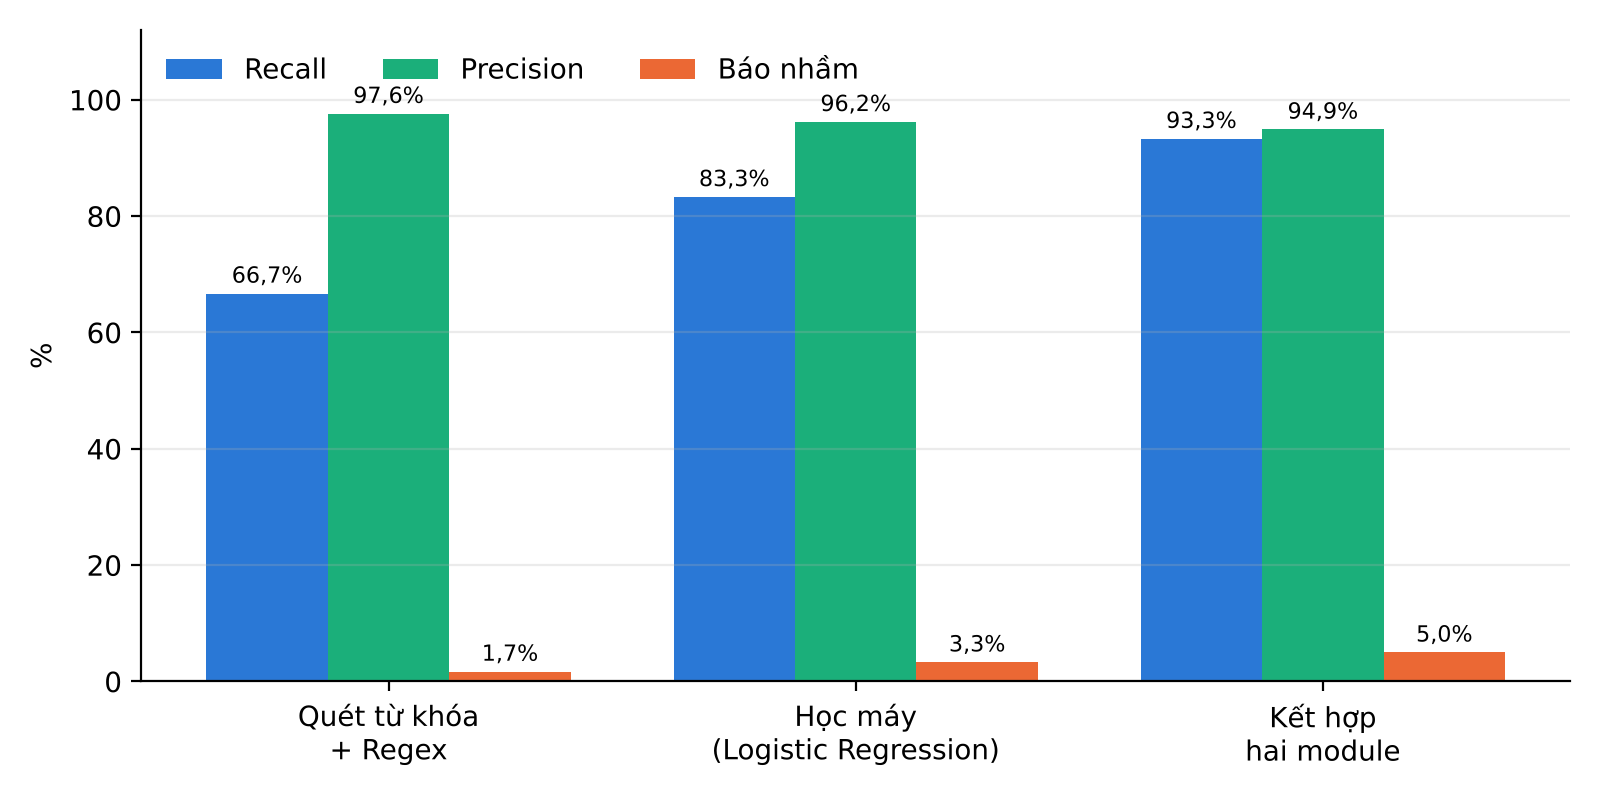
\includegraphics[width=0.85\textwidth]{figures/ket_qua_E1.png}
\caption{So sánh ba cách trên bộ kiểm tra 120 tin}
\label{fig:5.2}
\end{figure}

Về tốc độ, công cụ quét 46.000 tin mô phỏng trong khoảng 25 giây, tức gần 2.000 tin mỗi giây. Nếu một người đọc tay mất 30 giây cho mỗi tin, cùng khối lượng đó cần khoảng 383 giờ công, tương đương 48 ngày làm việc. Con số 46.000 lấy theo cỡ số gian hàng cơ quan điều tra công bố, nhưng đây là tin mô phỏng, không đại diện cho các gian hàng thật.

\paragraph{Demo trực tiếp}

Ô thử trực tiếp trong notebook cho phép nhập một tin bất kỳ và xem quyết định ngay. Ba tin dùng khi thuyết trình:

{\small\setstretch{1.1}
\begin{table}[H]
\centering
\caption{Kết quả demo trực tiếp}\label{tab:5.10}
\begin{tabularx}{\textwidth}{>{\hsize=1.099\hsize\raggedright\arraybackslash}X>{\hsize=0.548\hsize\raggedright\arraybackslash}X>{\hsize=1.353\hsize\raggedright\arraybackslash}X}
\toprule
\textbf{Tin nhập} & \textbf{Quyết định} & \textbf{Lý do công cụ đưa ra} \\
\midrule
Pass d.a.t.a khách mua bảo hiểm 5k số, mẫu 0912345678, 0987654321 & CHẶN (mua bán dữ liệu, điểm 0,95) & Từ khóa “data”, “data khách”; có mẫu dữ liệu cá nhân gồm 2 số điện thoại \\
Cho thuê sim nhận 0tp theo lượt, giao mã trong 30 giây. LH 0912345678 & CHẶN (dịch vụ xác thực hộ, điểm 0,81) & Từ khóa “otp”, “sim nhận”, “thuê sim”; “0tp” đã được chuẩn hóa thành “otp” \\
Khóa học nhận diện tin nhắn OTP giả mạo, phòng tránh lừa đảo. LH 0901222333 & CHO PHÉP (điểm 0,27) & Có từ “OTP” nhưng bị trừ điểm vì ngữ cảnh hợp lệ (“khóa học”); một số điện thoại liên hệ không bị tính là dữ liệu cá nhân \\
\bottomrule
\end{tabularx}
\end{table}}

\begin{figure}[H]
\centering
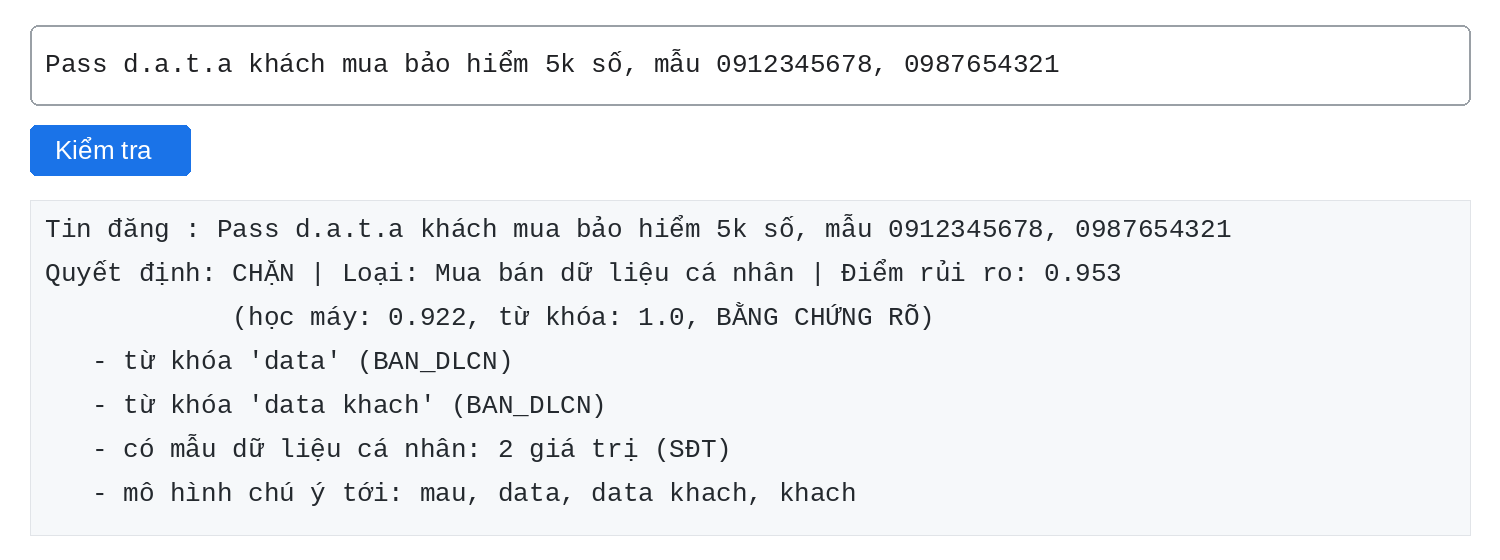
\includegraphics[width=0.95\textwidth]{figures/demo_truc_tiep.png}
\caption{Ô thử trực tiếp trong notebook với tin thứ nhất}
\label{fig:5.3}
\end{figure}

Mỗi tin bị gắn cờ được ghi vào nhật ký bằng chứng gồm thời điểm, quyết định, loại vi phạm, điểm rủi ro, lý do, nội dung đã che dữ liệu cá nhân (ví dụ “091*****78”) và mã băm SHA-256 của nội dung gốc để chứng minh nội dung không bị sửa sau khi ghi nhận. Nhật ký xuất ra file CSV và là đầu vào cho quy trình xử lý ở~\ref{sec:5.2.2}.

\paragraph{Tuân thủ khi triển khai thực tế}

Demo chỉ dùng dữ liệu tự tạo nên không xử lý dữ liệu cá nhân thật. Khi chạy trên tin đăng thật, công cụ vừa xử lý dữ liệu cá nhân của người bán và của những người có dữ liệu bị rao bán, vừa là một hệ thống trí tuệ nhân tạo. Vì vậy công cụ phải đáp ứng Luật Bảo vệ dữ liệu cá nhân 2025~\cite{luat-bvdlcn-2025}, Nghị định 356/2025/NĐ-CP~\cite{nd356-2025}, Luật Trí tuệ nhân tạo 2025~\cite{luat-ai-2025} và Nghị định 142/2026/NĐ-CP~\cite{nd142-2026}. Bảng dưới đây nêu từng yêu cầu và cách công cụ đáp ứng.

{\small\setstretch{1.1}
\begin{xltabular}{\textwidth}{>{\hsize=0.62\hsize\raggedright\arraybackslash}X>{\hsize=0.78\hsize\raggedright\arraybackslash}X>{\hsize=1.6\hsize\raggedright\arraybackslash}X}
\caption{Yêu cầu pháp lý khi triển khai công cụ phát hiện tin đăng}\label{tab:5.tuanthu}\\
\toprule
\textbf{Yêu cầu} & \textbf{Căn cứ} & \textbf{Cách đáp ứng} \\
\midrule
\endfirsthead
\toprule
\textbf{Yêu cầu} & \textbf{Căn cứ} & \textbf{Cách đáp ứng} \\
\midrule
\endhead
\bottomrule
\endlastfoot
Có căn cứ và đúng mục đích xử lý & Luật BVDLCN 2025: khoản 1 Điều 19, khoản 1 Điều 30; Nghị định 356/2025: Điều 19 & Chỉ quét tin đăng để phát hiện vi phạm, theo yêu cầu hoặc phối hợp với cơ quan có thẩm quyền; không dùng dữ liệu quét được cho mục đích khác. Lập hồ sơ đánh giá tác động xử lý dữ liệu cá nhân trước khi vận hành. \\
Dữ liệu huấn luyện hợp pháp & Luật Trí tuệ nhân tạo 2025: khoản 3 Điều 7 & Huấn luyện bằng dữ liệu tự tạo hoặc tin đăng đã khử nhận dạng; không dùng dữ liệu rò rỉ làm dữ liệu huấn luyện. \\
Mô hình không lưu dữ liệu cá nhân & Luật BVDLCN 2025: khoản 3 Điều 30 & Thay mọi dãy chữ số bằng một ký hiệu chung trước khi huấn luyện, để từ vựng của mô hình không chứa mảnh số điện thoại hay số CCCD. Mã hóa và phân quyền truy cập file mô hình. \\
Bảo vệ kết quả suy luận & Nghị định 356/2025: khoản 2 Điều 10 & Kết luận “gian hàng X có dấu hiệu bán dữ liệu” gắn với một người cụ thể nên cũng là dữ liệu cá nhân. Nhật ký bằng chứng chỉ lưu nội dung đã che và mã băm, chỉ người duyệt được xem, và có thời hạn lưu. \\
Con người quyết định cuối cùng & Luật Trí tuệ nhân tạo 2025: khoản 2 Điều 4, khoản 4 Điều 7 & CHẶN chỉ tạm ẩn tin và chuyển người duyệt xác nhận. Công cụ không tự gỡ tin hay khóa tài khoản. \\
Minh bạch và khiếu nại & Nghị định 356/2025: khoản 3 Điều 10; Luật Trí tuệ nhân tạo 2025: Điều 14 & Thông báo cho người bán rằng tin đăng được quét tự động, gửi kèm lý do bị gắn cờ (danh sách lý do do công cụ xuất ra) và kênh khiếu nại. \\
Phân loại rủi ro trước khi dùng & Luật BVDLCN 2025: khoản 4 Điều 30; Luật Trí tuệ nhân tạo 2025: Điều 9; Nghị định 142/2026: Điều 5 & Công cụ không tạo nội dung, không tương tác trực tiếp với công chúng, và người duyệt ra quyết định cuối, nên có cơ sở xếp vào mức rủi ro thấp. Trước khi dùng vẫn phải đối chiếu với Danh mục hệ thống trí tuệ nhân tạo rủi ro cao. \\
\end{xltabular}}

Nhóm đã thử bước thay chữ số trên notebook. Sau khi thay, từ vựng của mô hình không còn đặc trưng nào chứa từ ba chữ số liền nhau trở lên. Recall của riêng module học máy giảm từ 83,3\% xuống 80,0\%, còn kết quả của cách kết hợp hai module không đổi (recall 93,3\%, báo nhầm 5,0\%), vì số điện thoại và số CCCD vẫn do biểu thức chính quy nhận diện.

Quyền không tham gia xử lý tự động theo khoản 3 Điều 10 Nghị định 356/2025 khó áp dụng cho việc kiểm duyệt tin đăng bắt buộc trên sàn. Pháp luật hiện chưa quy định rõ trường hợp này.

\subsubsection{PoC tài liệu cho giải pháp 4 và 6: Bộ 3P xử lý sàn “chợ dữ liệu”}\label{sec:5.2.2}

PoC này cụ thể hóa giải pháp 4 và 6 theo cách tiếp cận 3P (Policy -- Process -- Procedure). Theo bài giảng về tuân thủ của môn học~\cite{lpsc-l6}, hệ thống quản lý an ninh thông tin của một tổ chức gồm chính sách, quy trình và thủ tục, và ba tầng này phải đối ứng với luật, quy định, hợp đồng bên ngoài. Ví dụ phân biệt: chính sách nêu điều phải đạt (“thông tin công ty trên máy tính phải được trả lại”), còn thủ tục nêu cách làm cụ thể (“phỏng vấn khi nghỉ việc và cách thu hồi tài liệu nhạy cảm”). PoC dùng ba tầng như sau:

{\small\setstretch{1.1}
\begin{table}[H]
\centering
\caption{Ba tầng 3P của PoC}\label{tab:5.3p}
\begin{tabularx}{\textwidth}{>{\raggedright\arraybackslash}l>{\hsize=0.8\hsize\raggedright\arraybackslash}X>{\hsize=1.2\hsize\raggedright\arraybackslash}X}
\toprule
\textbf{Tầng} & \textbf{Trả lời câu hỏi} & \textbf{Tài liệu trong PoC} \\
\midrule
Chính sách (Policy) & Phải đạt điều gì, theo căn cứ nào & Sáu cam kết: Đăng ký, Hàng cấm, Gỡ tin, Lưu trữ, Phối hợp theo vòng đời tin đăng; Giáo dục xuyên suốt (bảng~\ref{tab:5.cs}, \ref{tab:5.csdk}) \\
Quy trình (Process) & Gồm những bước nào, theo thứ tự nào & Luồng A, luồng B của nền tảng; phía cơ quan: bộ tiêu chí (bảng~\ref{tab:5.11}) và năm bước xử lý (hình~\ref{fig:5.4}) \\
Thủ tục (Procedure) & Ở mỗi bước: ai làm, làm gì, trong bao lâu & Thủ tục luồng A, B kèm ví dụ áp vào taphoammo (bảng~\ref{tab:5.tt}, \ref{tab:5.ttb}) và biểu mẫu tố giác (bảng~\ref{tab:5.12}) \\
\bottomrule
\end{tabularx}
\end{table}}

PoC nhắm vào ba thách thức ở chương 4 mà giải pháp 4 (Kiểm soát người bán) và giải pháp 6 (Phối hợp xử lý) phụ trách: Hạ tầng ở nước ngoài, Vỏ bọc doanh nghiệp và Dữ liệu nằm ở nhiều bên. Căn cứ là khung pháp luật hiện hành như đã nêu ở mục~\ref{sec:2.2.3}: Luật An ninh mạng 2025~\cite{luat-anm-2025}, Luật Bảo vệ dữ liệu cá nhân 2025~\cite{luat-bvdlcn-2025}, Nghị định 327/2026/NĐ-CP~\cite{nd327-2026} và Nghị định 333/2026/NĐ-CP~\cite{nd333-2026} (hai nghị định có hiệu lực từ 19/8/2026). PoC không áp ngược các văn bản này cho hành vi của taphoammo.net trước đó. Cảnh báo và nhật ký bằng chứng từ công cụ ở~\ref{sec:5.2.1} là một nguồn đầu vào của quy trình.

\paragraph{Tầng 1 -- Chính sách}

Sáu cam kết dưới đây là chính sách mà một nền tảng có gian hàng (sàn thương mại điện tử, chợ tài nguyên số) phải công bố và tuân thủ. Mỗi cam kết lấy nguyên ý từ một nghĩa vụ hoặc điều cấm trong luật. Thay vì đánh số, mỗi chính sách được gọi bằng một từ khóa và xếp theo vòng đời của một tin đăng trên sàn: đăng ký tài khoản, đăng tin, lưu trữ dữ liệu, và khi cơ quan chức năng có yêu cầu. Chính sách Giáo dục không gắn với một giai đoạn mà áp dụng xuyên suốt cho người vận hành các bước đó; chính sách này xuất phát từ nghĩa vụ tuyên truyền, phổ biến pháp luật của nhà cung cấp dịch vụ (điểm g khoản 2 Điều 6 Nghị định 327/2026).

{\small\setstretch{1.1}
\begin{table}[H]
\centering
\caption{Chính sách của nền tảng theo vòng đời một tin đăng}\label{tab:5.cs}
\begin{tabularx}{\textwidth}{>{\raggedright\arraybackslash}l>{\hsize=1.2\hsize\raggedright\arraybackslash}X>{\raggedright\arraybackslash}l>{\hsize=1.1\hsize\raggedright\arraybackslash}X>{\hsize=0.7\hsize\raggedright\arraybackslash}X}
\toprule
\textbf{Chính sách} & \textbf{Nội dung cam kết} & \textbf{Ai} & \textbf{Căn cứ} & \textbf{Thách thức} \\
\midrule
\multicolumn{5}{l}{\textit{Giai đoạn đăng ký}} \\
\textbf{Đăng ký} & Xác thực thông tin khi đăng ký tài khoản; chỉ tài khoản đã xác thực mới được đăng tin & Nền tảng & Luật ANM 2025: điểm a khoản 2 Điều 25; NĐ 333/2026: điểm a, d khoản 2 Điều 16 & Dữ liệu nằm ở nhiều bên (xác định người đứng sau gian hàng) \\
\multicolumn{5}{l}{\textit{Giai đoạn đăng tin}} \\
\textbf{Hàng cấm} & Không đăng bán dữ liệu cá nhân, tài khoản số, dịch vụ xác thực tài khoản hộ & Người dùng & Luật BVDLCN 2025: khoản 6 Điều 7; Luật ANM 2025: điểm h khoản 2 Điều 7, điểm g khoản 4 Điều 13 & Vỏ bọc doanh nghiệp (danh tính hợp lệ không làm hàng hóa hợp lệ) \\
\textbf{Gỡ tin} & Chủ động phát hiện, ngăn chặn và kịp thời gỡ bỏ tin xâm phạm bí mật cá nhân, đời sống riêng tư & Nền tảng & Luật ANM 2025: điểm b khoản 2 Điều 15 & Vỏ bọc doanh nghiệp \\
\multicolumn{5}{l}{\textit{Giai đoạn lưu trữ}} \\
\textbf{Lưu trữ} & Lưu dữ liệu người dùng tại Việt Nam (tối thiểu 24 tháng); nhật ký hệ thống truy xuất được ít nhất 12 tháng & Nền tảng & Luật ANM 2025: khoản 3 Điều 25; NĐ 333/2026: khoản 1, 2 Điều 19, khoản 1 Điều 20, điểm c khoản 6 Điều 16 & Hạ tầng ở nước ngoài \\
\multicolumn{5}{l}{\textit{Khi cơ quan chức năng có yêu cầu}} \\
\textbf{Phối hợp} & Chỉ định đầu mối phối hợp, tiếp nhận yêu cầu khẩn cấp theo chế độ thường trực 24/24 giờ; cung cấp thông tin, gỡ bỏ trong thời hạn luật định & Nền tảng & NĐ 327/2026: khoản 2 Điều 14; Luật ANM 2025: điểm a, b khoản 2 Điều 25 & Dữ liệu nằm ở nhiều bên \\
\multicolumn{5}{l}{\textit{Xuyên suốt các giai đoạn}} \\
\textbf{Giáo dục} & Phổ biến pháp luật và các thủ đoạn vi phạm mới cho người duyệt, đầu mối phối hợp, người vận hành hệ thống & Nền tảng & NĐ 327/2026: điểm g, điểm a khoản 2 Điều 6; NĐ 329/2026: khoản 1, điểm đ khoản 4 Điều 6~\cite{nd329-2026} & Vỏ bọc doanh nghiệp \\
\bottomrule
\end{tabularx}
\end{table}}

\paragraph{Vì sao là sáu chính sách này: PoC giải quyết gì, không giải quyết gì}

Chín thách thức ở chương 4 không cùng một loại, nên không cùng một cách giải. Bảng~\ref{tab:5.pv} xếp chúng theo cách giải, dựa trên bảng~\ref{tab:5.6}. PoC tài liệu chỉ nhận ba thách thức mà lời giải là quy định ai làm gì, trong bao lâu; đó đúng là nội dung của chính sách, quy trình và thủ tục.

{\small\setstretch{1.1}
\begin{table}[H]
\centering
\caption{Thách thức nào PoC tài liệu giải quyết}\label{tab:5.pv}
\begin{tabularx}{\textwidth}{>{\hsize=1.1\hsize\raggedright\arraybackslash}X>{\hsize=1.0\hsize\raggedright\arraybackslash}X>{\hsize=0.9\hsize\raggedright\arraybackslash}X}
\toprule
\textbf{Thách thức (chương 4)} & \textbf{Giải bằng} & \textbf{Giải pháp (mục~\ref{sec:5.1})} \\
\midrule
Hạ tầng ở nước ngoài; Vỏ bọc doanh nghiệp; Dữ liệu nằm ở nhiều bên & \textbf{Quy định ai làm gì, trong bao lâu: PoC tài liệu 3P} & 4 -- Kiểm soát người bán; 6 -- Phối hợp xử lý \\
Khối lượng lớn; Cách viết lách bộ lọc & Công cụ phát hiện & 1 -- Phát hiện tin có dấu hiệu vi phạm (demo) \\
Nhiều văn bản, hiệu lực khác nhau theo thời gian; Ranh giới trách nhiệm giữa người bán và sàn & Phân tích pháp lý & 5 -- Ma trận trách nhiệm pháp lý (đề xuất) \\
Tài khoản đổi chủ; Dữ liệu dễ sao chép & Bên khác, không phải sàn: nền tảng gốc của tài khoản, bên kiểm soát dữ liệu & 2 -- Bảo vệ tài khoản trên nền tảng gốc; 3 -- Truy nguồn rò rỉ dữ liệu (đề xuất) \\
\bottomrule
\end{tabularx}
\end{table}}

Với ba thách thức PoC nhận, bảng~\ref{tab:5.csdk} đi từ dữ kiện đã công bố ở chương 3 tới chính sách tương ứng. Cụm từ in đậm trong cột dữ kiện là chỗ thể hiện thách thức.

{\small\setstretch{1.1}
\begin{table}[H]
\centering
\caption{Thách thức, dữ kiện vụ việc và chính sách tương ứng}\label{tab:5.csdk}
\begin{tabularx}{\textwidth}{>{\hsize=0.7\hsize\raggedright\arraybackslash}X>{\hsize=1.3\hsize\raggedright\arraybackslash}X>{\hsize=1.1\hsize\raggedright\arraybackslash}X>{\hsize=0.9\hsize\raggedright\arraybackslash}X}
\toprule
\textbf{Thách thức} & \textbf{Dữ kiện} & \textbf{Chuyện gì đã xảy ra} & \textbf{Chính sách} \\
\midrule
Vỏ bọc doanh nghiệp & Công ty có đăng ký, \textbf{có kiểm duyệt người bán}, nhưng vẫn bán dữ liệu cá nhân, tài khoản, dịch vụ xác thực (mục~\ref{sec:3.1}, \ref{sec:3.2.1}) & Người bán được kiểm tra; hàng hóa không được kiểm tra, không bị gỡ & Hàng cấm, Gỡ tin, Giáo dục (riêng Đăng ký là chưa đủ) \\
Hạ tầng ở nước ngoài & Hơn 1,35 triệu tài khoản; \textbf{máy chủ ở nước ngoài}, tên miền đi thuê (mục~\ref{sec:3.2.2}) & Dữ liệu người dùng không có bản lưu trong nước; cơ quan điều tra nêu việc này gây khó truy vết & Lưu trữ \\
Dữ liệu nằm ở nhiều bên & Tin đăng, thanh toán, hạ tầng, quảng cáo nằm ở \textbf{sàn, ngân hàng hoặc ví điện tử, nhà cung cấp máy chủ, nền tảng quảng cáo} (mục~\ref{sec:3.2.3}, \ref{sec:3.2.4}, \ref{sec:4.3}) & Thông tin về người đứng sau gian hàng nằm rải rác ở nhiều bên, không có đầu mối, không có thời hạn & Đăng ký, Phối hợp \\
-- & Việc chạy quảng cáo (mục~\ref{sec:3.2.3}); làm trung gian thanh toán (mục~\ref{sec:3.2.4}) & -- & Ngoài phạm vi PoC; đối chiếu ở chương~\ref{sec:7} và pháp luật thanh toán \\
\bottomrule
\end{tabularx}
\end{table}}

\paragraph{Tầng 2 -- Quy trình: hai luồng của nền tảng}

Chính sách, quy trình và thủ tục là tài liệu của cùng một tổ chức. Quy trình của PoC vì vậy được viết cho nền tảng, gồm hai luồng:

\begin{itemize}
\item \textbf{Luồng A -- nền tảng tự kiểm soát:} Đăng ký $\rightarrow$ Duyệt tin $\rightarrow$ Gỡ tin $\rightarrow$ Lưu trữ. Luồng này thực hiện các chính sách Đăng ký, Hàng cấm, Gỡ tin và Lưu trữ. Cảnh báo từ công cụ ở~\ref{sec:5.2.1} là đầu vào của bước Duyệt tin. Chính sách Giáo dục áp dụng xuyên suốt cả hai luồng cho người thực hiện các bước.
\item \textbf{Luồng B -- nền tảng phối hợp với cơ quan:} Nhận yêu cầu $\rightarrow$ Xác thực $\rightarrow$ Thực hiện $\rightarrow$ Phản hồi. Luồng này thực hiện chính sách Phối hợp. Khoản 2 Điều 14 Nghị định 327/2026 áp dụng cho chủ quản hệ thống thông tin, nhà cung cấp dịch vụ và cơ quan, tổ chức có liên quan~\cite{nd327-2026}, nên cùng luồng này áp dụng cho các bên khác đang giữ dữ liệu của vụ việc như ngân hàng hoặc ví điện tử, nhà cung cấp máy chủ, nền tảng quảng cáo (thách thức Dữ liệu nằm ở nhiều bên).
\end{itemize}

\paragraph{Tầng 2 -- Quy trình phía cơ quan chức năng: bộ tiêu chí nhận diện “chợ dữ liệu”}

Khi chính nhà vận hành cố ý vi phạm như taphoammo.net, nền tảng sẽ không tự áp dụng luồng A. Phần việc lúc này thuộc cơ quan chức năng: nhận diện sàn, chuyển đúng thẩm quyền và gửi yêu cầu vào luồng B của sàn và của các bên giữ dữ liệu. Bộ tiêu chí giúp người kiểm tra quyết định một sàn có cần được xem xét như một “chợ dữ liệu” hay không. Mỗi tiêu chí xây từ một đặc điểm đã công bố của taphoammo~\cite{bca-2026}.

{\small\setstretch{1.1}
\begin{table}[H]
\centering
\caption{Bộ tiêu chí nhận diện “chợ dữ liệu”, căn cứ theo luật hiện hành}\label{tab:5.11}
\begin{tabularx}{\textwidth}{>{\raggedright\arraybackslash}l>{\hsize=0.6\hsize\raggedright\arraybackslash}X>{\hsize=1.15\hsize\raggedright\arraybackslash}X>{\hsize=1.25\hsize\raggedright\arraybackslash}X>{\hsize=1.0\hsize\raggedright\arraybackslash}X}
\toprule
\textbf{STT} & \textbf{Tiêu chí} & \textbf{Dấu hiệu kiểm tra} & \textbf{Căn cứ} & \textbf{Đặc điểm tương ứng ở taphoammo} \\
\midrule
1 & Hàng hóa đăng bán & Đăng bán dữ liệu cá nhân, thông tin tài khoản số, dịch vụ xác thực tài khoản hộ; có thể dùng công cụ ở~\ref{sec:5.2.1} để sàng lọc & Luật BVDLCN 2025: khoản 6 Điều 7; Luật ANM 2025: điểm g khoản 4 Điều 13; NĐ 330/2026: điểm c khoản 2 Điều 14 & Đăng bán công khai dữ liệu cá nhân, tài khoản mạng xã hội và thư điện tử \\
2 & Thu phí trung gian & Sàn nhận, giữ, chuyển tiền thay người mua, người bán và thu phí trên mỗi giao dịch & NĐ 330/2026: điểm b khoản 2 Điều 14; NĐ 340/2025: khoản 6 Điều 31 & Thu phí 3--5\% mỗi giao dịch \\
3 & Kiểm duyệt người bán & Sàn có duyệt gian hàng nhưng vẫn để hàng hóa vi phạm tồn tại & NĐ 327/2026: khoản 10 Điều 10; NĐ 330/2026: điểm e khoản 2 Điều 15 & Có kiểm duyệt người bán \\
4 & Quảng cáo đa nền tảng & Sàn được quảng cáo trên mạng xã hội, công cụ tìm kiếm & NĐ 330/2026: điểm d khoản 3 Điều 14; NĐ 327/2026: điểm a khoản 2 Điều 6 (nền tảng quảng cáo phải rà soát) & Quảng cáo trên Facebook, Telegram, TikTok, Instagram, Google \\
5 & Hạ tầng ở nước ngoài & Doanh nghiệp trong nước đặt máy chủ ở nước ngoài, không có bản lưu dữ liệu người dùng trong nước & Luật ANM 2025: khoản 3 Điều 25; NĐ 333/2026: khoản 2 Điều 19; NĐ 330/2026: điểm c khoản 2 Điều 29, điểm a khoản 1 Điều 33 & Máy chủ ở nước ngoài, thuê tên miền \\
6 & Vỏ bọc doanh nghiệp & Có đăng ký doanh nghiệp nhưng ngành nghề không khớp hàng hóa thực tế & NĐ 330/2026: điểm đ khoản 1 Điều 53; NĐ 327/2026: khoản 10 Điều 10 & Đứng tên Công ty TNHH Phát triển Công nghệ số HCT \\
\bottomrule
\end{tabularx}
\end{table}}

Mỗi tiêu chí dựa trên một điều cấm, nghĩa vụ hoặc hành vi bị xử phạt trong khung pháp luật hiện hành~\cite{luat-anm-2025,luat-bvdlcn-2025,nd327-2026,nd330-2026,nd333-2026,nd340-2025}. Cách đánh giá là quy tắc do nhóm đề xuất cho PoC: tiêu chí 1 (hàng hóa đăng bán) là điều kiện bắt buộc. Sàn thỏa tiêu chí 1 và ít nhất hai tiêu chí khác thì được chuyển sang quy trình xử lý; sàn chỉ thỏa tiêu chí 1 được đưa vào danh sách theo dõi. Áp vào taphoammo.net, cột cuối của bảng~\ref{tab:5.11} cho thấy sàn thỏa cả sáu tiêu chí bằng dữ kiện đã công bố.

\paragraph{Tầng 2 -- Quy trình phía cơ quan chức năng: năm bước xử lý khi một sàn bị nhận diện}

Quy trình nối tiếp kết quả của công cụ ở~\ref{sec:5.2.1} và cụ thể hóa giải pháp 6 ở~\ref{sec:5.1}. Bộ tiêu chí ở trên được dùng tại bước sàng lọc. Bảng~\ref{tab:5.ttcq} ghi căn cứ của từng bước và sự kiện tương ứng trong vụ việc. Các mốc vụ việc diễn ra trước khi Luật An ninh mạng 2025 và các nghị định hướng dẫn có hiệu lực; cột cuối chỉ cho biết sự kiện thật ứng với từng bước, không có nghĩa các điều khoản này đã được áp dụng.

{\small\setstretch{1.1}
\begin{xltabular}{\textwidth}{>{\raggedright\arraybackslash}l>{\hsize=1.2\hsize\raggedright\arraybackslash}X>{\hsize=0.95\hsize\raggedright\arraybackslash}X>{\hsize=0.85\hsize\raggedright\arraybackslash}X}
\caption{Quy trình phía cơ quan chức năng: căn cứ và đối chiếu vụ việc}\label{tab:5.ttcq}\\
\toprule
\textbf{Bước} & \textbf{Cơ quan làm gì} & \textbf{Căn cứ} & \textbf{Trong vụ việc} \\
\midrule
\endfirsthead
\toprule
\textbf{Bước} & \textbf{Cơ quan làm gì} & \textbf{Căn cứ} & \textbf{Trong vụ việc} \\
\midrule
\endhead
\bottomrule
\endlastfoot
1. Tiếp nhận & Nhận cảnh báo (kể cả từ công cụ ở~\ref{sec:5.2.1}), tố giác của tổ chức, cá nhân và nhà cung cấp dịch vụ, theo biểu mẫu ở bảng~\ref{tab:5.12} & NĐ 327/2026: khoản 5 Điều 10, khoản 1 Điều 11, khoản 1 Điều 14; NĐ 329/2026: điểm d khoản 2 Điều 5 & 6/2025: lập chuyên án sau khi phát hiện qua nắm tình hình trên không gian mạng \\
2. Sàng lọc, xác minh & Chấm sáu tiêu chí; xác minh tài khoản số, địa chỉ mạng, đường dẫn & NĐ 327/2026: khoản 2 Điều 9, khoản 3 Điều 11 & Thỏa 6/6 tiêu chí (bảng~\ref{tab:5.11}) \\
3. Thu thập dữ liệu điện tử & Dữ liệu điện tử không bị can thiệp, thay đổi; quá trình thu thập được ghi biên bản, hình ảnh và có thể lặp lại; che dữ liệu cá nhân khi lưu hồ sơ & NĐ 333/2026: khoản 3 Điều 12 & 2/2026: khám xét, thu giữ máy tính và dữ liệu điện tử \\
4. Áp dụng biện pháp & Yêu cầu cung cấp thông tin, xóa bỏ thông tin (luồng B của sàn và các bên giữ dữ liệu) và kiểm tra việc chấp hành; yêu cầu phong tỏa tài khoản số, tạm dừng giao dịch; đình chỉ hệ thống thông tin, đề nghị Bộ Khoa học và Công nghệ thu hồi tên miền (trường hợp cấp bách: yêu cầu trực tiếp, văn bản chậm nhất 24 giờ sau đó); doanh nghiệp Việt Nam phối hợp ngăn chặn dịch vụ qua biên giới vi phạm & NĐ 327/2026: khoản 3, 4 Điều 9; NĐ 333/2026: khoản 2 Điều 11, khoản 2, 4 Điều 13, khoản 3 Điều 14 & Áp vào: yêu cầu ngân hàng, ví điện tử phong tỏa tài khoản nhận tiền của sàn; đề nghị thu hồi tên miền taphoammo.net \\
5. Chuyển thẩm quyền, xử lý & Bộ Công an là đầu mối chủ trì với hoạt động dân sự, kinh tế; hành vi thuộc chuyên ngành khác (ví dụ trung gian thanh toán) áp dụng nghị định chuyên ngành; có dấu hiệu tội phạm thì chuyển hồ sơ truy cứu trách nhiệm hình sự & NĐ 333/2026: điểm a khoản 5 Điều 14; NĐ 329/2026: điểm a khoản 3 Điều 9; NĐ 330/2026: khoản 3 Điều 1, khoản 4 Điều 4; Luật ANM 2025: điểm n khoản 1 Điều 5 & 25/12/2025: khởi tố vụ án; 7/2026: công bố khởi tố 3 bị can về tội theo Điều 288 Bộ luật Hình sự \\
\end{xltabular}}

\begin{figure}[H]
\centering
% Quy trình xử lý khi một sàn bị nhận diện (bản sơ bộ, Người 5 có thể thay)
\setstretch{1}
\begin{tikzpicture}[font=\small, node distance=0.4cm,
  box/.style={draw, rounded corners=2pt, align=center, minimum height=1.3cm, text width=2.3cm, fill=blue!7},
  arr/.style={-{Stealth[length=2mm]}, thick}]
  \node[box] (a) {Tiếp nhận};
  \node[box, right=of a] (b) {Sàng lọc theo\\bộ tiêu chí};
  \node[box, right=of b] (c) {Bảo toàn\\chứng cứ};
  \node[box, right=of c] (d) {Chuyển đúng\\thẩm quyền};
  \node[box, right=of d] (e) {Theo dõi và\\phản hồi};
  \foreach \u/\v in {a/b, b/c, c/d, d/e} \draw[arr] (\u) -- (\v);
\end{tikzpicture}

\caption{Quy trình phía cơ quan chức năng khi một sàn bị nhận diện}
\label{fig:5.4}
\end{figure}

\paragraph{Tầng 3 -- Thủ tục cho từng bước}

Thủ tục ghi rõ ở mỗi bước ai làm, làm gì và trong thời hạn nào. Các thời hạn trong bảng đều lấy từ văn bản pháp luật; bước nào luật không quy định thời hạn thì ghi “không quy định”. Cột cuối áp thủ tục vào taphoammo.net bằng các dữ kiện đã công bố~\cite{bca-2026}, để thấy mỗi thủ tục trông ra sao trong một vụ việc cụ thể.

{\small\setstretch{1.1}
\begin{xltabular}{\textwidth}{>{\raggedright\arraybackslash}l>{\hsize=1.25\hsize\raggedright\arraybackslash}X>{\hsize=0.6\hsize\raggedright\arraybackslash}X>{\hsize=0.8\hsize\raggedright\arraybackslash}X>{\hsize=1.05\hsize\raggedright\arraybackslash}X}
\caption{Thủ tục luồng A -- nền tảng tự kiểm soát}\label{tab:5.tt}\\
\toprule
\textbf{Bước} & \textbf{Thủ tục (ai, làm gì)} & \textbf{Thời hạn} & \textbf{Căn cứ} & \textbf{Áp vào taphoammo} \\
\midrule
\endfirsthead
\toprule
\textbf{Bước} & \textbf{Thủ tục (ai, làm gì)} & \textbf{Thời hạn} & \textbf{Căn cứ} & \textbf{Áp vào taphoammo} \\
\midrule
\endhead
\bottomrule
\endlastfoot
Đăng ký & Nền tảng xác thực tài khoản bằng số điện thoại di động tại Việt Nam, hoặc bằng số định danh cá nhân; tài khoản chưa xác thực không được đăng tin & Khi đăng ký tài khoản & NĐ 333/2026: điểm a, b, d khoản 2 Điều 16 & Sàn đã có kiểm duyệt người bán; riêng bước này không ngăn được hàng cấm \\
Duyệt tin & Công cụ ở~\ref{sec:5.2.1} chấm mỗi tin mới (CHẶN, CHUYỂN NGƯỜI DUYỆT, CHO PHÉP); người duyệt quyết định với tin bị gắn cờ & Không quy định & Luật ANM 2025: điểm b khoản 2 Điều 15; Luật BVDLCN 2025: khoản 6 Điều 7 & Gian hàng bán tài khoản Facebook, TikTok, Telegram, Instagram, thư điện tử thuộc nhóm “mua bán tài khoản” mà công cụ gắn cờ \\
Gỡ tin & Ghi nhật ký xử lý tin, lưu bằng chứng (ảnh chụp, mã băm) rồi gỡ tin. Tài khoản đăng từ 03 tin vi phạm trở lên trong 30 ngày bị hạn chế hiển thị hoặc khóa tạm thời tối đa 60 ngày; từ 10 tin trở lên trong 90 ngày thì tối đa 180 ngày & “Kịp thời” & Luật ANM 2025: điểm b khoản 2 Điều 15; NĐ 333/2026: điểm d khoản 4, điểm b khoản 6 Điều 16 & Sàn có hơn 46.000 gian hàng; gian hàng đăng lặp lại tin vi phạm bị khóa theo các ngưỡng này \\
Lưu trữ & Lưu tại Việt Nam: thông tin cá nhân, tên tài khoản, thời gian sử dụng, địa chỉ IP đăng nhập, đăng xuất gần nhất, số điện thoại gắn với tài khoản. Nhật ký gồm tài khoản, thời gian đăng nhập, đăng xuất, địa chỉ IP, cổng nguồn và nhật ký xử lý tin đăng & Dữ liệu tối thiểu 24 tháng; nhật ký ít nhất 12 tháng & NĐ 333/2026: khoản 1, 2 Điều 19, khoản 1 Điều 20, điểm b, c khoản 6 Điều 16 & Hơn 1,35 triệu tài khoản trên máy chủ ở nước ngoài: phải có bản lưu các dữ liệu này trong nước \\
Giáo dục & Nền tảng (bộ phận thường trực bảo vệ an ninh mạng, nếu có) phổ biến pháp luật và các thủ đoạn vi phạm rà soát được cho người duyệt, đầu mối, người vận hành & Không quy định & NĐ 327/2026: điểm g, điểm a khoản 2 Điều 6; NĐ 329/2026: khoản 1, điểm đ khoản 4 Điều 6 & Nội dung lấy từ vụ việc: dữ liệu cá nhân, tài khoản mạng xã hội, thư điện tử, “dịch vụ xác thực tài khoản”; người bán đã xác thực không làm hàng hóa hợp pháp \\
\end{xltabular}}

{\small\setstretch{1.1}
\begin{xltabular}{\textwidth}{>{\raggedright\arraybackslash}l>{\hsize=1.2\hsize\raggedright\arraybackslash}X>{\hsize=0.65\hsize\raggedright\arraybackslash}X>{\hsize=0.8\hsize\raggedright\arraybackslash}X>{\hsize=1.05\hsize\raggedright\arraybackslash}X}
\caption{Thủ tục luồng B -- nền tảng phối hợp với cơ quan}\label{tab:5.ttb}\\
\toprule
\textbf{Bước} & \textbf{Thủ tục (ai, làm gì)} & \textbf{Thời hạn} & \textbf{Căn cứ} & \textbf{Áp vào taphoammo} \\
\midrule
\endfirsthead
\toprule
\textbf{Bước} & \textbf{Thủ tục (ai, làm gì)} & \textbf{Thời hạn} & \textbf{Căn cứ} & \textbf{Áp vào taphoammo} \\
\midrule
\endhead
\bottomrule
\endlastfoot
Nhận yêu cầu & Đầu mối phối hợp của nền tảng nhận yêu cầu bằng văn bản giấy, văn bản điện tử, đường dây nóng; yêu cầu khẩn cấp theo chế độ thường trực & 24/24 giờ & NĐ 327/2026: khoản 1 Điều 12, khoản 2 Điều 14 & Yêu cầu của lực lượng chuyên trách về các gian hàng bán dữ liệu cá nhân đến đầu mối của sàn \\
Xác thực & Xác thực chủ thể yêu cầu; bảo mật thông tin được cung cấp & Không quy định & NĐ 333/2026: điểm b khoản 3 Điều 16 & Chỉ gửi dữ liệu người dùng khi xác nhận yêu cầu đúng là của lực lượng chuyên trách thuộc Bộ Công an \\
Thực hiện & Cung cấp thông tin người dùng; ngăn chặn chia sẻ, xóa thông tin, gỡ dịch vụ theo yêu cầu & Cung cấp chậm nhất 24 giờ (khẩn cấp 03 giờ); gỡ bỏ chậm nhất 24 giờ (khẩn cấp 06 giờ) & Luật ANM 2025: điểm a, b khoản 2 Điều 25; NĐ 333/2026: điểm c khoản 3, điểm b khoản 4 Điều 16 & Với mỗi chủ gian hàng: tên tài khoản, thời gian sử dụng dịch vụ, thông tin thanh toán, địa chỉ IP (danh mục ở điểm d khoản 2 Điều 25 Luật ANM 2025) \\
Phản hồi & Thực hiện và phản hồi kết quả xử lý & Theo thời hạn trong yêu cầu & NĐ 327/2026: khoản 2 Điều 14 & Báo lại tin nào đã gỡ, dữ liệu nào đã cung cấp, vào thời điểm nào \\
\end{xltabular}}

Luồng A cùng các chính sách Đăng ký, Hàng cấm, Gỡ tin xử lý thách thức Vỏ bọc doanh nghiệp: kiểm tra danh tính người bán và kiểm tra hàng hóa là hai bước riêng. Chính sách Lưu trữ và bước thu hồi tên miền phía cơ quan (Điều 13 Nghị định 333/2026) xử lý thách thức Hạ tầng ở nước ngoài: không với tới được máy chủ ở nước ngoài, nhưng dữ liệu người dùng Việt Nam có bản lưu trong nước và tên miền có thể bị tạm ngừng, thu hồi. Luồng B xử lý thách thức Dữ liệu nằm ở nhiều bên: mỗi bên giữ dữ liệu có một đầu mối, có phương thức phối hợp và có thời hạn.

\paragraph{Biểu mẫu tiếp nhận tố giác}

Biểu mẫu là phần thủ tục của bước tiếp nhận trong quy trình phía cơ quan chức năng, gồm các trường sau:

{\small\setstretch{1.1}
\begin{table}[H]
\centering
\caption{Các trường của biểu mẫu tiếp nhận tố giác}\label{tab:5.12}
\begin{tabularx}{\textwidth}{>{\hsize=0.541\hsize\raggedright\arraybackslash}X>{\hsize=1.459\hsize\raggedright\arraybackslash}X>{\raggedright\arraybackslash}l}
\toprule
\textbf{Trường} & \textbf{Nội dung} & \textbf{Bắt buộc} \\
\midrule
Người tố giác & Họ tên và cách liên hệ; cho phép tố giác ẩn danh & Không \\
Đối tượng bị tố giác & Địa chỉ sàn, gian hàng hoặc đường dẫn tin đăng & Có \\
Loại hành vi nghi ngờ & Chọn trong bảy hành vi ở Chương 3, kèm mô tả ngắn & Có \\
Thời điểm phát hiện & Ngày, giờ phát hiện & Có \\
Bằng chứng & Ảnh chụp màn hình, đường dẫn; không gửi kèm dữ liệu cá nhân bị rò rỉ & Có \\
Cam kết & Thông tin cung cấp là trung thực; không gửi dữ liệu cá nhân ngoài phạm vi cần thiết & Có \\
Phần cơ quan tiếp nhận ghi & Mã hồ sơ, người tiếp nhận, kết quả sàng lọc theo bộ tiêu chí, đơn vị được chuyển hồ sơ & Có \\
\bottomrule
\end{tabularx}
\end{table}}


\paragraph{Kiểm tra độ phủ theo McCumber Cube}

McCumber Cube~\cite{lpsc-l1} có ba trục vẽ từ một gốc chung: tính chất cần bảo vệ (Confidentiality, Integrity, Availability), trạng thái của thông tin (Storage, Processing, Transmission) và nhóm biện pháp (Policy, Education, Technology). Các biện pháp được áp dụng đồng thời, bổ trợ nhau, và phải cân nhắc đánh đổi. Nhóm dùng ba trục này để kiểm tra bộ 3P và công cụ ở~\ref{sec:5.2.1} có bỏ trống chiều nào không:

{\small\setstretch{1.1}
\begin{table}[H]
\centering
\caption{Đối chiếu PoC với ba trục của McCumber Cube}\label{tab:5.mc}
\begin{tabularx}{\textwidth}{>{\raggedright\arraybackslash}l>{\raggedright\arraybackslash}l>{\hsize=1.3\hsize\raggedright\arraybackslash}X>{\hsize=0.7\hsize\raggedright\arraybackslash}X}
\toprule
\textbf{Trục} & \textbf{Thành phần} & \textbf{Phần của PoC đáp ứng} & \textbf{Ghi chú} \\
\midrule
\multirow{3}{*}{CIA} & Confidentiality & Hàng cấm, Gỡ tin: chặn việc đăng bán dữ liệu cá nhân, tài khoản & \\
 & Integrity & Gỡ tin (nhật ký xử lý, mã băm); bước thu thập dữ liệu điện tử phía cơ quan: dữ liệu không bị thay đổi & \\
 & Availability & Lưu trữ, Phối hợp: dữ liệu lưu trong nước, cung cấp trong 24 giờ & Cho cơ quan có thẩm quyền \\
\midrule
\multirow{3}{*}{Trạng thái} & Storage & Lưu trữ: lưu tại Việt Nam, nhật ký 12 tháng & \\
 & Processing & Đăng ký, Duyệt tin, công cụ ở~\ref{sec:5.2.1}: xác thực, quét tin đăng & \\
 & Transmission & Luồng B: xác thực chủ thể yêu cầu, bảo mật thông tin được cung cấp & \\
\midrule
\multirow{3}{*}{Biện pháp} & Policy & Sáu chính sách ở bảng~\ref{tab:5.cs} & \\
 & Technology & Công cụ ở~\ref{sec:5.2.1}, mã băm, xác thực tài khoản & \\
 & Education & Chính sách Giáo dục: phổ biến pháp luật, thủ đoạn vi phạm cho người duyệt, đầu mối, người vận hành & NĐ 327/2026 điểm g khoản 2 Điều 6 \\
\bottomrule
\end{tabularx}
\end{table}}

Trục Education được đáp ứng bằng chính sách Giáo dục. Luật không quy định tần suất phổ biến, nên thủ tục ghi “không quy định”; nội dung lấy từ các thủ đoạn mà nền tảng rà soát được (điểm a khoản 2 Điều 6 Nghị định 327/2026).

% chuong6.tex — sửa nội dung chương ở đây
\section{Đánh giá và kết luận}\label{sec:6}

\subsection{Đánh giá}\label{sec:6.1}

\subsubsection{Đánh giá công cụ phát hiện tin đăng}\label{sec:6.1.1}

\textbf{Mỗi module có đóng góp riêng.} Module quét từ khóa + Regex chính xác (precision 97,6\%, báo nhầm 1,7\%) nhưng chỉ bắt được 66,7\% tin vi phạm: tin viết bằng từ ngữ ngoài bộ từ khóa sẽ lọt qua, ví dụ “Kho Telegram account” hay “Có Gmail tạo sẵn, nhận giao theo lô”. Module học máy bắt rộng hơn (recall 83,3\%) nhờ nhận ra cách viết chưa có trong bộ từ khóa, nhưng bỏ sót một số tin dùng từ lóng như “pass tài khoản mạng xã hội” hay “thuê SIM nhận mã”.

\textbf{Kết hợp hai module cải thiện rõ rệt.} Recall tăng lên 93,3\%, vì hai module bỏ sót những tin khác nhau. Đổi lại, báo nhầm tăng lên 5,0\% (3 trên 60 tin hợp lệ), và cả 3 tin này chỉ bị chuyển người duyệt, không bị chặn thẳng. Với mục tiêu sàng lọc, đánh đổi này chấp nhận được: bỏ sót một tin vi phạm gây hại nhiều hơn việc một nhân viên phải xem lại một tin hợp lệ.

\textbf{Liên hệ với thách thức.} Với thách thức về khối lượng tin đăng, công cụ quét 46.000 tin trong khoảng 25 giây thay cho khoảng 48 ngày làm việc nếu đọc tay; người kiểm tra chỉ cần xem các tin bị gắn cờ. Với thách thức về tin ngụy trang, bộ kiểm tra có nhiều tin ngụy trang (“d.a.t.a”, “0tp”, “v1a”) và công cụ vẫn nhận ra nhờ bước chuẩn hóa chữ.

\textbf{Hạn chế của demo:}

\begin{itemize}
\item Dữ liệu huấn luyện và kiểm tra đều do nhóm tự tạo, nên số liệu minh họa phương pháp, không phải hiệu năng trên một sàn thật.
\item Công cụ chưa hiểu ngữ cảnh: tin hợp lệ như “Nhận tư vấn xác minh danh tính khách hàng đúng quy trình KYC” hay “Dịch vụ nhập dữ liệu khách hàng đã được doanh nghiệp cho phép xử lý” vẫn bị chuyển người duyệt.
\item Người bán sẽ đổi cách viết khi biết bị lọc, nên bộ từ khóa và mô hình phải được cập nhật thường xuyên.
\item Công cụ chỉ đọc nội dung tin đăng; giao dịch chuyển sang Telegram, Zalo hoặc dữ liệu gửi riêng sau khi mua nằm ngoài tầm quét.
\item Công cụ không thay người duyệt và không tự kết luận vi phạm.
\end{itemize}
\subsubsection{Đánh giá bộ tiêu chí và quy trình xử lý}\label{sec:6.1.2}

Áp bộ tiêu chí ở~\ref{sec:5.2.2} lên dòng thời gian vụ việc~\cite{bca-2026}:

{\small\setstretch{1.1}
\begin{table}[H]
\centering
\caption{Áp bộ tiêu chí lên dòng thời gian vụ việc}\label{tab:6.13}
\begin{tabularx}{\textwidth}{>{\raggedright\arraybackslash}l>{\hsize=0.591\hsize\raggedright\arraybackslash}X>{\hsize=1.409\hsize\raggedright\arraybackslash}X}
\toprule
\textbf{Mốc} & \textbf{Sự kiện} & \textbf{Ý nghĩa với bộ tiêu chí} \\
\midrule
Cuối 2021 & Sàn bắt đầu hoạt động & Hàng hóa vi phạm được đăng bán công khai trên trang (tiêu chí 1). Mô hình giữ tiền, thu phí 3–5\% (tiêu chí 2) là cách sàn vận hành theo mô tả của cơ quan điều tra \\
6/2025 & Lập chuyên án sau khi phát hiện qua nắm tình hình trên không gian mạng & Cho thấy dấu hiệu của sàn nhận ra được từ bên ngoài, qua nội dung đăng bán (tiêu chí 1) và quảng cáo (tiêu chí 4) \\
25/12/2025 & Quyết định khởi tố vụ án hình sự & Không thêm tiêu chí mới \\
2/2026 & Khám xét, thu giữ máy tính và dữ liệu điện tử & Các đặc điểm vận hành bên trong như kiểm duyệt người bán (tiêu chí 3) và vỏ bọc doanh nghiệp (tiêu chí 6) được làm rõ qua điều tra \\
7/2026 & Công bố vụ việc & Cả sáu đặc điểm được công bố chính thức, kể cả máy chủ ở nước ngoài (tiêu chí 5) \\
\bottomrule
\end{tabularx}
\end{table}}

Hai tiêu chí quan trọng nhất, tiêu chí 1 và 4, đều quan sát được từ bên ngoài mà không cần quyền điều tra: chỉ cần xem nội dung đăng bán và quảng cáo của sàn. Nếu bộ tiêu chí và công cụ phát hiện tin đăng được áp dụng thường xuyên, các dấu hiệu này có cơ hội được ghi nhận sớm hơn mốc lập chuyên án. Đây là suy luận của nhóm; dữ kiện công bố không cho biết cơ quan chức năng đã biết gì và từ khi nào, nên bài không khẳng định vụ việc chắc chắn bị phát hiện từ năm đầu.

Bộ tiêu chí cũng cần không gắn cờ nhầm các sàn hợp pháp. Thử áp với một sàn sản phẩm số hợp pháp giả định, bán key phần mềm bản quyền và khóa học, có thu phí trung gian và quảng cáo trên mạng xã hội: sàn này thỏa tiêu chí 2, 4 và có thể cả tiêu chí 3, nhưng không thỏa tiêu chí 1 nên không bị chuyển sang quy trình xử lý. Việc đặt tiêu chí 1 làm điều kiện bắt buộc giúp bộ tiêu chí không gắn cờ những sàn chỉ giống taphoammo ở mô hình kinh doanh.

Biểu mẫu tố giác có đủ thông tin tối thiểu (đối tượng, loại hành vi, thời điểm, bằng chứng) để cơ quan tiếp nhận sàng lọc theo bộ tiêu chí và chuyển hồ sơ. Quy trình và biểu mẫu mới được xây dựng trên giấy, chưa được thử với một cơ quan hay nền tảng thật.

\subsubsection{Đánh giá khi áp dụng bộ 3P vào vụ việc}\label{sec:6.1.3p}

Mục này so sánh dữ kiện của vụ taphoammo.net với những gì bộ 3P ở~\ref{sec:5.2.2} yêu cầu, theo ba thách thức mà PoC phụ trách. Cột “thực tế” chỉ dùng dữ kiện đã công bố~\cite{bca-2026,cand-2026}; cột “khi áp dụng” chỉ dùng thời hạn và nghĩa vụ ghi trong văn bản~\cite{luat-anm-2025,nd327-2026,nd333-2026}. Vì các văn bản này có hiệu lực sau thời gian sàn hoạt động, đây là phép so sánh giả định để đánh giá giải pháp, không phải đánh giá trách nhiệm của các bị can.

{\small\setstretch{1.1}
\begin{xltabular}{\textwidth}{>{\hsize=0.7\hsize\raggedright\arraybackslash}X>{\hsize=1.1\hsize\raggedright\arraybackslash}X>{\hsize=1.2\hsize\raggedright\arraybackslash}X>{\hsize=1.0\hsize\raggedright\arraybackslash}X}
\caption{Thực tế vụ việc và khi áp dụng bộ 3P}\label{tab:6.3p}\\
\toprule
\textbf{Thách thức} & \textbf{Thực tế vụ việc} & \textbf{Khi áp dụng bộ 3P} & \textbf{Phần chưa giải quyết} \\
\midrule
\endfirsthead
\toprule
\textbf{Thách thức} & \textbf{Thực tế vụ việc} & \textbf{Khi áp dụng bộ 3P} & \textbf{Phần chưa giải quyết} \\
\midrule
\endhead
\bottomrule
\endlastfoot
Hạ tầng ở nước ngoài & Máy chủ ở nước ngoài, tên miền đi thuê; cơ quan điều tra nêu việc này gây khó truy vết; khoảng 8 tháng từ lập chuyên án (6/2025) đến khám xét (2/2026) & Lưu trữ: dữ liệu người dùng Việt Nam lưu trong nước ít nhất 24 tháng, nhật ký 12 tháng. Phía cơ quan: tạm ngừng, thu hồi tên miền theo Điều 13 NĐ 333/2026; trường hợp khẩn cấp có văn bản trong 24 giờ & Máy chủ đặt ở nước ngoài vẫn cần hợp tác quốc tế và nhà cung cấp hạ tầng \\
Vỏ bọc doanh nghiệp & Sàn đứng tên công ty có đăng ký, có kiểm duyệt người bán nhưng hàng hóa vi phạm vẫn được đăng bán & Đăng ký tách khỏi Hàng cấm, Gỡ tin (luồng A): kiểm tra danh tính và kiểm tra hàng hóa là hai bước; tiêu chí 6 đối chiếu ngành nghề với hàng hóa thực tế & Một nhà vận hành cố ý vi phạm sẽ không tự tuân thủ chính sách; khi đó phải dựa vào tiêu chí 1 và 4, quan sát được từ bên ngoài \\
Dữ liệu nằm ở nhiều bên & Tin đăng, thanh toán, hạ tầng, quảng cáo nằm ở sàn, ngân hàng hoặc ví, nhà cung cấp máy chủ và nền tảng quảng cáo & Phối hợp (luồng B): một đầu mối thường trực 24/24 giờ; cung cấp thông tin trong 24 giờ (khẩn cấp 03 giờ); gỡ bỏ trong 24 giờ (khẩn cấp 06 giờ) & Thủ tục giữa các bộ ngoài Bộ Công an (Bộ Công Thương, Ngân hàng Nhà nước) chưa có thời hạn trong PoC \\
\end{xltabular}}

Thay đổi rõ nhất là các bước xử lý có thời hạn tính bằng giờ thay vì không có mốc nào. Trong vụ việc, các mốc công bố tính bằng tháng và năm: sàn hoạt động khoảng 3,5 năm trước khi bị lập chuyên án và thêm khoảng 8 tháng đến khi khám xét. Bộ 3P không rút ngắn được phần điều tra hình sự, nhưng đặt thời hạn cho những việc nền tảng và các bên nắm dữ liệu phải làm khi được yêu cầu. Với một nhà vận hành cố ý vi phạm như taphoammo.net, giá trị chính của tầng chính sách là làm thước đo: không lưu dữ liệu trong nước, không ngăn chặn hàng hóa vi phạm đều là vi phạm hành chính có chế tài riêng (chương~\ref{sec:7}), nên có thể xử lý từ sớm mà không phải chờ đủ yếu tố cấu thành tội phạm.

\paragraph{Cân bằng giữa các yếu tố}

Khi đánh đổi an ninh (security trade-offs) có hai góc nhìn: góc kỹ thuật (hiệu năng, chức năng; khả năng sử dụng) và góc quản lý (sự hài lòng của người dùng; quyền truy cập; ngân sách). Bảng dưới đây đánh giá ở mức định tính từng biện pháp theo ba phía đó.

{\small\setstretch{1.1}
\begin{table}[H]
\centering
\caption{Đánh đổi của từng biện pháp}\label{tab:6.tradeoff}
\begin{tabularx}{\textwidth}{>{\hsize=0.75\hsize\raggedright\arraybackslash}X>{\hsize=1.05\hsize\raggedright\arraybackslash}X>{\hsize=1.1\hsize\raggedright\arraybackslash}X>{\hsize=1.1\hsize\raggedright\arraybackslash}X}
\toprule
\textbf{Biện pháp} & \textbf{An ninh (CIA)} & \textbf{Kỹ thuật} & \textbf{Quản lý} \\
\midrule
Đăng ký: xác thực người bán & Tăng tính bí mật: khó mở gian hàng ẩn danh & Thêm bước khi đăng ký; tài khoản chưa xác thực chỉ được đọc (NĐ 333/2026 điểm d khoản 2 Điều 16) & Chi phí xác thực; người bán hợp pháp có thể không hài lòng \\
Lưu trữ: lưu dữ liệu trong nước & Tăng tính sẵn sàng của dữ liệu cho cơ quan có thẩm quyền & Phải có hạ tầng lưu trữ trong nước & Chi phí hạ tầng \\
Công cụ ở~\ref{sec:5.2.1} & Bắt 93,3\% tin vi phạm trên bộ kiểm tra & Quét 46.000 tin trong khoảng 25 giây; báo nhầm 5,0\% & Cần người duyệt các tin bị gắn cờ \\
Phối hợp: thời hạn 24 giờ & Thông tin và tin vi phạm được xử lý nhanh & Cần quy trình truy xuất dữ liệu kịp thời & Cần đầu mối trực 24/24 giờ \\
Bảo toàn chứng cứ & Tăng tính toàn vẹn của chứng cứ & Lưu ảnh chụp, mã băm, nhật ký & Thời gian ghi biên bản; chi phí lưu trữ \\
\bottomrule
\end{tabularx}
\end{table}}

Không biện pháp nào tăng an ninh mà không tốn chi phí ở phía kỹ thuật hoặc quản lý. Vì vậy PoC giữ con người ở bước quyết định (công cụ chỉ gắn cờ), dùng thời hạn do luật định thay vì tự đặt thời hạn ngắn hơn, và để trống những bước luật không quy định thời hạn.

\subsubsection{Giới hạn chung của giải pháp}\label{sec:6.1.3}

\begin{itemize}
\item Giải pháp 2, 3 và 5 mới ở mức đề xuất, chưa được hiện thực hay thử nghiệm.
\item Thách thức về hạ tầng đặt ở nước ngoài phụ thuộc hợp tác quốc tế và nhà cung cấp hạ tầng, ngoài tầm của các giải pháp trong bài.
\item Các giải pháp hỗ trợ phát hiện và xử lý; trách nhiệm pháp lý cụ thể vẫn do cơ quan có thẩm quyền xác định.
\end{itemize}
\subsection{Kết luận}\label{sec:6.2}

Phần kết luận trả lời lần lượt ba câu hỏi nghiên cứu ở mục~\ref{sec:2.1}.

\textbf{Câu hỏi 1: Hoạt động của sàn taphoammo.net vi phạm những quy định nào?} Chương 3 xác định bảy hành vi. Ba hành vi thuộc nội dung khởi tố là mua bán dữ liệu cá nhân, mua bán tài khoản mạng xã hội và thư điện tử, và cung cấp dịch vụ xác thực tài khoản hộ, đối chiếu với khoản 5 Điều 7 Luật An toàn thông tin mạng 2015, Nghị định 13/2023/NĐ-CP và Điều 288 Bộ luật Hình sự. Bốn hành vi còn lại là kết luận của nhóm từ dữ kiện đã công bố: kiểm duyệt người bán nhưng vẫn để hàng hóa vi phạm tồn tại, đặt máy chủ ở nước ngoài, quảng cáo dịch vụ bị cấm, và làm trung gian thanh toán cho giao dịch bị cấm. Vụ án chưa có bản án, nên các bị can vẫn được suy đoán vô tội.

\textbf{Câu hỏi 2: Điều gì khiến việc áp dụng luật chưa ngăn chặn được sớm?} Các hành vi này đã bị cấm từ trước khi sàn hoạt động, nhưng việc áp dụng gặp chín thách thức nêu ở chương 4. Về kỹ thuật, khối lượng tin đăng lớn và cách viết ngụy trang khiến đọc thủ công không theo kịp; tài khoản và dữ liệu dễ chuyển tay, khó truy nguồn; hạ tầng đặt ở nước ngoài. Về pháp lý, một hành vi liên quan nhiều văn bản có hiệu lực khác nhau theo thời gian, và trách nhiệm của sàn với người bán chưa được tách bạch. Về quản trị, đăng ký doanh nghiệp tạo vỏ bọc hợp pháp và dữ liệu điều tra nằm ở nhiều bên.

\textbf{Câu hỏi 3: Cần biện pháp gì để phát hiện và ngăn chặn các sàn tương tự?} Nhóm đề xuất sáu giải pháp gắn với từng thách thức. Giải pháp 1 đã được kiểm chứng bằng demo: kết hợp quét từ khóa + Regex với học máy phát hiện 93,3\% tin vi phạm trên bộ kiểm tra với tỉ lệ báo nhầm 5,0\%, và quét 46.000 tin trong khoảng 25 giây. Giải pháp 4 và 6 có PoC tài liệu theo cách tiếp cận 3P: sáu chính sách có căn cứ luật, quy trình năm bước kèm bộ tiêu chí nhận diện “chợ dữ liệu”, và thủ tục từng bước với thời hạn lấy từ Luật An ninh mạng 2025, Nghị định 327/2026 và 333/2026, kèm biểu mẫu tố giác. Giải pháp 2, 3 và 5 dừng ở mức đề xuất.

\textbf{Hướng phát triển.} Thử công cụ phát hiện tin đăng trên dữ liệu thật do nền tảng cung cấp trong khuôn khổ được phép, bổ sung khả năng hiểu ngữ cảnh và câu phủ định, thử nghiệm quy trình phối hợp xử lý với một cơ quan hoặc nền tảng cụ thể, và xây dựng nội dung cụ thể cho chính sách Giáo dục (tài liệu phổ biến cho người duyệt và đầu mối phối hợp).


% chuong7.tex — phần mở rộng: đối chiếu hành vi với Luật An ninh mạng 2025 và Nghị định 330/2026
\section{Mở rộng: đối chiếu với Luật An ninh mạng 2025 và Nghị định 330/2026}\label{sec:7}

Chương 3 xét hành vi của taphoammo.net theo văn bản có hiệu lực tại thời điểm hành vi. Chương này trả lời một câu hỏi khác: nếu cùng các hành vi đó xảy ra khi Luật An ninh mạng 2025~\cite{luat-anm-2025} và Nghị định 330/2026/NĐ-CP~\cite{nd330-2026} đã có hiệu lực, thì khung pháp luật hiện hành gọi tên và xử phạt chúng ra sao. Mục đích là làm rõ khung hiện hành mà giải pháp ở chương 5 dựa vào, không phải áp ngược luật mới cho vụ việc. Các trích dẫn điều khoản lấy từ bản text của văn bản gốc trong thư mục \texttt{legal/}.

\subsection{Nguyên tắc áp dụng}\label{sec:7.1}

\begin{itemize}
\item \textbf{Hiệu lực.} Luật An ninh mạng 2025 có hiệu lực từ 1/7/2026; Luật An toàn thông tin mạng 2015 và Luật An ninh mạng 2018 hết hiệu lực từ cùng ngày (khoản 1, 2 Điều 44). Nghị định 330/2026 có hiệu lực từ 19/8/2026 (Điều 80).
\item \textbf{Không áp ngược.} Hành vi xảy ra trước 19/8/2026 áp dụng nghị định xử phạt có hiệu lực tại thời điểm vi phạm; chỉ áp dụng Nghị định 330/2026 nếu nghị định này không quy định trách nhiệm hoặc quy định nhẹ hơn (khoản 1 Điều 81).
\item \textbf{Hình sự loại trừ hành chính.} Hành vi có dấu hiệu tội phạm được chuyển hồ sơ truy cứu trách nhiệm hình sự (khoản 4 Điều 4). Ba bị can đã bị khởi tố theo Điều 288 Bộ luật Hình sự, nên các mức phạt dưới đây chỉ có ý nghĩa với người tham gia không bị truy cứu, hoặc với hành vi tương tự trong tương lai.
\item \textbf{Cách đọc mức phạt.} Ở Mục 1 đến Mục 5 Chương II (an ninh mạng), mức ghi trong điều là mức cho cá nhân, tổ chức chịu gấp hai lần; ở Mục 6 (bảo vệ dữ liệu cá nhân), mức ghi là mức cho tổ chức, cá nhân chịu một phần hai (khoản 1 Điều 7). Mức tối đa trong lĩnh vực an ninh mạng là 100 triệu đồng với cá nhân và 200 triệu đồng với tổ chức (khoản 3 Điều 7); với mua bán dữ liệu cá nhân là 10 lần khoản thu (điểm a khoản 4 Điều 7).
\item \textbf{Thời hiệu.} Thời hiệu xử phạt trong lĩnh vực an ninh mạng và bảo vệ dữ liệu cá nhân là 01 năm (khoản 1 Điều 3).
\end{itemize}

\subsection{Hành vi của nhà vận hành sàn}\label{sec:7.2}

Bảng dưới đây đặt các hành vi đã phân tích ở chương 3 cạnh điều cấm hoặc nghĩa vụ của Luật An ninh mạng 2025 và điều xử phạt của Nghị định 330/2026. Việc gắn hành vi với điều khoản là phân tích của nhóm.

{\small\setstretch{1.1}
\begin{xltabular}{\textwidth}{>{\hsize=1.0\hsize\raggedright\arraybackslash}X>{\hsize=0.95\hsize\raggedright\arraybackslash}X>{\hsize=0.85\hsize\raggedright\arraybackslash}X>{\hsize=1.2\hsize\raggedright\arraybackslash}X}
\caption{Hành vi của nhà vận hành sàn theo Luật An ninh mạng 2025 và Nghị định 330/2026}\label{tab:7.1}\\
\toprule
\textbf{Hành vi (mục ở chương 3)} & \textbf{Luật ANM 2025} & \textbf{NĐ 330/2026} & \textbf{Mức phạt tiền} \\
\midrule
\endfirsthead
\toprule
\textbf{Hành vi (mục ở chương 3)} & \textbf{Luật ANM 2025} & \textbf{NĐ 330/2026} & \textbf{Mức phạt tiền} \\
\midrule
\endhead
\bottomrule
\endlastfoot
Mua bán dữ liệu cá nhân, kể cả thông tin tài khoản số (3.1.1, 3.1.2) & Điểm h khoản 2 Điều 7; điểm g khoản 4 Điều 13 (và khoản 6 Điều 7 Luật BVDLCN 2025) & Khoản 1, 3 Điều 53 (Mục 6) & Từ 02 đến 10 lần khoản thu; nếu không có khoản thu: từ 70 triệu đến 3 tỷ đồng tùy số chủ thể dữ liệu và mức độ (tổ chức; cá nhân một phần hai) \\
Lập, vận hành, tiếp thị trực tuyến cho sàn trái phép (3.2.1, 3.2.3) & Điểm e khoản 4 Điều 13 & Điểm d khoản 3 Điều 14 & Cá nhân 20--30 triệu; tổ chức 40--60 triệu \\
Không kiểm duyệt, ngăn chặn, loại bỏ hành vi vi phạm trên hệ thống (3.2.1) & Điểm b khoản 2 Điều 15 & Điểm e khoản 2 Điều 15 & Cá nhân 20--30 triệu; tổ chức 40--60 triệu \\
Không lưu dữ liệu người dùng Việt Nam tại Việt Nam (3.2.2) & Khoản 3 Điều 25; khoản 7 Điều 41 & Điểm c khoản 2 Điều 29; điểm a khoản 1 Điều 33 & Điều 29: cá nhân 50--70 triệu, tổ chức 100--140 triệu. Điều 33: cá nhân 30--50 triệu, tổ chức 60--100 triệu \\
Cung cấp dịch vụ nhận tin nhắn, cuộc gọi để xác thực tài khoản (3.1.3) & Điểm g khoản 4 Điều 13 & Điểm c khoản 2 Điều 14, chỉ khi là tài khoản có chức năng giao dịch tài chính & Cá nhân 10--20 triệu; tổ chức 20--40 triệu \\
Trung gian thanh toán cho giao dịch hàng cấm (3.2.4) & Không có điều tương ứng trực tiếp & Điểm b khoản 2 Điều 14 (dùng tài khoản số làm công cụ trung gian nhận, chuyển tiền khi không được cấp phép); nếu là hành vi cung ứng dịch vụ trung gian thanh toán thì áp dụng nghị định chuyên ngành (khoản 3 Điều 1): khoản 6 Điều 31 Nghị định 340/2025/NĐ-CP~\cite{nd340-2025} & Điều 14: cá nhân 10--20 triệu; tổ chức 20--40 triệu. Nghị định 340/2025: cá nhân 150--250 triệu; tổ chức 300--500 triệu \\
\end{xltabular}}

Kèm theo phạt tiền, Nghị định 330/2026 quy định các biện pháp như: buộc hủy, xóa toàn bộ dữ liệu cá nhân đã mua bán, buộc nộp lại khoản thu, buộc thông báo cho chủ thể dữ liệu bị ảnh hưởng (khoản 5 Điều 53); buộc nộp lại số lợi bất hợp pháp (điểm d khoản 4 Điều 15); buộc lưu trữ dữ liệu tại Việt Nam (điểm a khoản 3 Điều 33); buộc thu hồi tên miền do thực hiện hành vi vi phạm (khoản 3 Điều 5).

\subsection{Người bán và người mua trên sàn}\label{sec:7.3}

Phạm vi đề tài tập trung vào nhà vận hành sàn (mục~\ref{sec:1.2}), nhưng Nghị định 330/2026 có điều xử phạt riêng cho người bán và người mua. Bảng dưới đây chỉ liệt kê để đối chiếu.

{\small\setstretch{1.1}
\begin{table}[H]
\centering
\caption{Một số hành vi của người bán, người mua theo Nghị định 330/2026}\label{tab:7.2}
\begin{tabularx}{\textwidth}{>{\hsize=1.4\hsize\raggedright\arraybackslash}X>{\hsize=0.8\hsize\raggedright\arraybackslash}X>{\hsize=0.8\hsize\raggedright\arraybackslash}X}
\toprule
\textbf{Hành vi} & \textbf{NĐ 330/2026} & \textbf{Cá nhân / tổ chức} \\
\midrule
Đưa lên mạng thông tin thuộc bí mật cá nhân, đời sống riêng tư (người bán) & Điểm a khoản 1 Điều 13 & 10--20 / 20--40 triệu \\
Bán, cho thuê tài khoản số có chức năng giao dịch tài chính của mình (người bán) & Khoản 1 Điều 14 & 5--10 / 10--20 triệu \\
Dùng trái phép thông tin của người khác để đăng ký tài khoản số có chức năng giao dịch tài chính & Điểm a khoản 2 Điều 14 & 10--20 / 20--40 triệu \\
Sử dụng thông tin đăng nhập, quyền truy cập tài khoản số không đúng quy định (người mua) & Điểm c khoản 3 Điều 14 & 20--30 / 40--60 triệu \\
Sử dụng tài khoản mạng xã hội của người khác không được chủ tài khoản đồng ý (người mua) & Điểm e khoản 5 Điều 14 & 50--70 / 100--140 triệu \\
\bottomrule
\end{tabularx}
\end{table}}

\subsection{Nhận xét}\label{sec:7.4}

\begin{itemize}
\item Hành vi cốt lõi là mua bán dữ liệu cá nhân không bị phạt ở các mục an ninh mạng (Mục 1 đến Mục 5) mà ở Điều 53, thuộc mục bảo vệ dữ liệu cá nhân, với mức phạt tính theo khoản thu. Đây là điều khoản duy nhất trong bảng~\ref{tab:7.1} có mức phạt tăng theo quy mô giao dịch.
\item Các nghĩa vụ mà chính sách Đăng ký, Gỡ tin, Lưu trữ ở mục~\ref{sec:5.2.2} dựa vào (xác thực tài khoản, ngăn chặn hành vi vi phạm, lưu dữ liệu trong nước) đều có điều xử phạt tương ứng ở Điều 15, 29 và 33 Nghị định 330/2026. Vì vậy, vi phạm chính sách của bộ 3P cũng là căn cứ xử lý hành chính.
\item Với vụ taphoammo.net, các hành vi đã bị khởi tố hình sự và xảy ra trước khi hai văn bản có hiệu lực. Chương này không thay đổi kết luận ở chương 3.
\end{itemize}


\clearpage
% Danh mục tài liệu tham khảo. Trích dẫn trong bài bằng \cite{khóa}; số thứ tự tự đánh.
\begin{thebibliography}{99}

\bibgroup{Văn bản pháp luật}
\bibitem{luat-attm-2015} Quốc hội (2015). \textit{Luật An toàn thông tin mạng}, số 86/2015/QH13. \href{https://hethongphapluat.com/luat-an-toan-thong-tin-mang-2015/dieu-7}{Điều 7}.
\bibitem{blhs-2015} Quốc hội (2015, sửa đổi 2017). \textit{Bộ luật Hình sự}, số 100/2015/QH13. \href{https://hethongphapluat.com/bo-luat-hinh-su-2015/dieu-288}{Điều 288}.
\bibitem{luat-anm-2018} Quốc hội (2018). \textit{Luật An ninh mạng}, số 24/2018/QH14. \href{https://hethongphapluat.com/luat-an-ninh-mang-2018/dieu-26}{Điều 26}.
\bibitem{nd53-2022} Chính phủ (2022). \textit{Nghị định 53/2022/NĐ-CP quy định chi tiết một số điều của Luật An ninh mạng}. Tóm tắt tại \href{https://lsvn.vn/tu-01102022-du-lieu-nguoi-dung-internet-tai-viet-nam-se-duoc-luu-tru1661052929-a122807.html}{LSVN}.
\bibitem{nd13-2023} Chính phủ (2023). \textit{Nghị định 13/2023/NĐ-CP về bảo vệ dữ liệu cá nhân}. \href{https://hethongphapluat.com/nghi-dinh-13-2023-nd-cp-ve-bao-ve-du-lieu-ca-nhan/khoan-3-dieu-2}{Điều 2 khoản 3}, \href{https://hethongphapluat.com/nghi-dinh-13-2023-nd-cp-ve-bao-ve-du-lieu-ca-nhan/dieu-3}{Điều 3}.
\bibitem{luat-bvdlcn-2025} Quốc hội (2025). \textit{Luật Bảo vệ dữ liệu cá nhân}, số 91/2025/QH15. \href{https://vanban.chinhphu.vn/?docid=214590&pageid=27160}{Hồ sơ chính thức}; \href{https://congbaocdn.chinhphu.vn/CongBaoCP/CongBao/2025/7/45574/57723-1-971-972.pdf}{bản Công báo, Điều 7, 8, 23}; mức phạt tại \href{https://lsvn.vn/mua-ban-du-lieu-ca-nhan-trai-phep-co-the-bi-phat-toi-10-lan-doanh-thu-a160473.html}{LSVN}.
\bibitem{nd356-2025} Chính phủ (2025). \textit{Nghị định 356/2025/NĐ-CP quy định chi tiết Luật Bảo vệ dữ liệu cá nhân}. \href{https://congbao.cdnchinhphu.vn/180507251028987904/2026/1/17/356signed-1768638052103952849513.pdf}{Bản Công báo}; tóm tắt tại \href{https://luatvietan.vn/diem-moi-cua-nghi-dinh-356-2025-so-voi-nghi-dinh-13-2023-ve-huong-dan-bao-ve-du-lieu-ca-nhan.html}{Luật Việt An}.
\bibitem{luat-qc-2012} Quốc hội (2012). \textit{Luật Quảng cáo}, số 16/2012/QH13. \href{https://hethongphapluat.com/luat-quang-cao-2012/dieu-8}{Điều 8}; \href{https://hrspring.vn/van-ban-luat/luat-quang-cao-sua-doi-2025-so-75-2025-qh15}{Luật sửa đổi số 75/2025/QH15}.
\bibitem{nd52-2013} Chính phủ (2013, sửa đổi 2021). \textit{Nghị định 52/2013/NĐ-CP về thương mại điện tử}, sửa đổi bởi Nghị định 85/2021/NĐ-CP. Phân tích tại \href{https://lsvn.vn/bao-dam-quyen-loi-cua-nguoi-tieu-dung-khi-mua-hang-tren-san-giao-dich-thuong-mai-dien-tu-1707211306-a140810.html}{LSVN}.
\bibitem{vbhn-tmdt-2020} Bộ Công Thương (2020). \textit{Văn bản hợp nhất quy định về thương mại điện tử}, \href{https://congbao.chinhphu.vn/tai-ve-van-ban-so-20-vbhn-bct-30960-30438?format=pdf}{Công báo 2020}, Điều 4.
\bibitem{nd52-2024} Chính phủ (2024). \textit{Nghị định 52/2024/NĐ-CP về thanh toán không dùng tiền mặt}. \href{https://vbpl.vn/nganhangnhanuoc/Pages/vbpq-toanvan.aspx?ItemID=167087}{Toàn văn}; \href{https://pbgdpl.cantho.gov.vn/mot-so-hanh-vi-bi-cam-trong-thanh-toan-khong-dung-tien-mat-tu-ngay-0172024}{Điều 8}.
\bibitem{luat-anm-2025} Quốc hội (2025). \textit{Luật An ninh mạng}, số 116/2025/QH15. \href{https://vanban.chinhphu.vn/?classid=1&docid=216499&pageid=27160&typegroupid=3}{Hồ sơ chính thức}; \href{https://apolatlegal.com/vi/laws/luat-an-ninh-mang-2025-so-116-2025-qh15/}{Apolat Legal}; \href{https://hethongphapluat.com/luat-an-ninh-mang-2025/dieu-44}{Điều 44}.
\bibitem{luat-tmdt-2025} Quốc hội (2025). \textit{Luật Thương mại điện tử}, số 122/2025/QH15. \href{https://luatvietnam.vn/tin-van-ban-moi/da-co-luat-thuong-mai-dien-tu-2025-so-122-2025-qh15-186-106402-article.html}{LuatVietnam}.
\bibitem{luat-ai-2025} Quốc hội (2025). \textit{Luật Trí tuệ nhân tạo}, số 134/2025/QH15, hiệu lực từ 1/3/2026. \href{https://thuvienphapluat.vn/van-ban/EN/Cong-nghe-thong-tin/Law-134-2025-QH15-Artificial-Intelligence/689735/tieng-anh.aspx}{Bản tiếng Anh}; tóm tắt tại \href{https://apolatlegal.com/vi/laws/luat-tri-tue-nhan-tao-2025-so-134-2025-qh15/}{Apolat Legal}.
\bibitem{nd142-2026} Chính phủ (2026). \textit{Nghị định 142/2026/NĐ-CP hướng dẫn Luật Trí tuệ nhân tạo}, hiệu lực từ 1/5/2026. Tóm tắt tại \href{https://luatvietan.vn/nghi-dinh-142-2026-nd-cp-huong-dan-luat-tri-tue-nhan-tao.html}{Luật Việt An}.

\bibgroup{Thông tin chính thức và báo chí về vụ taphoammo.net}
\bibitem{bca-2026} Bộ Công an (14/7/2026). \href{https://www.bocongan.gov.vn/bai-viet/triet-pha-nhom-doi-tuong-van-hanh-website-mua-ban-du-lieu-ca-nhan-tai-khoan-mang-xa-hoi-rac-1784022194}{Triệt phá nhóm đối tượng vận hành website mua bán dữ liệu cá nhân, tài khoản mạng xã hội}.
\bibitem{cand-2026} Báo Công an Nhân dân (9/7/2026). \href{https://cand.vn/mua-ban-du-lieu-duoi-vo-boc-cua-cong-ty-khoi-nghiep-3-doi-tuong-bi-khoi-to-post816257.html}{Mua bán dữ liệu dưới vỏ bọc của công ty khởi nghiệp, 3 đối tượng bị khởi tố}.
\bibitem{vnn-2026} VietNamNet (10/7/2026). \href{https://vietnamnet.vn/cong-an-tp-ha-noi-khoi-to-3-nguoi-dieu-hanh-san-mua-ban-du-lieu-ca-nhan-2534474.html}{Công an TP Hà Nội khởi tố 3 người điều hành sàn mua bán dữ liệu cá nhân}.
\bibitem{hnm-2026} Hà Nội Mới (10/7/2026). \href{https://hanoimoi.vn/khoi-to-cac-doi-tuong-mua-ban-du-lieu-ca-nhan-thu-loi-tren-400-ty-dong-1211456.html}{Khởi tố các đối tượng mua bán dữ liệu cá nhân thu lời trên 400 tỷ đồng}.
\bibitem{k14-2026} Kenh14 (11/7/2026, tổng hợp từ Đời sống \& Pháp luật). \href{https://kenh14.vn/hang-tram-canh-sat-ap-vao-kham-xet-tai-3-tinh-thanh-khoi-to-giam-doc-dao-quang-huy-sn-1992-215260710160532629.chn}{Hàng trăm cảnh sát ập vào khám xét tại 3 tỉnh thành, khởi tố Giám đốc Đào Quang Huy}.
\bibitem{bpl-2026} Báo Pháp luật Việt Nam (14/7/2026). \href{https://baophapluat.vn/triet-pha-website-taphoammo-net-ban-trai-phep-du-lieu-ca-nhan-thu-loi-tu-he-thong-1-35-trieu-tai-khoan.html}{Triệt phá website taphoammo.net bán trái phép dữ liệu cá nhân}.
\bibitem{dtud-2026} Tạp chí Điện tử và Ứng dụng (14/7/2026). \href{https://dientuungdung.vn/vu-tap-hoa-mmo-he-lo-mang-toi-mua-ban-du-lieu-ca-nhan-16575.html}{Vụ Tạp Hóa MMO hé lộ mảng tối mua bán dữ liệu cá nhân}.

\bibgroup{Hướng dẫn của cơ quan nhà nước}
\bibitem{cuc-tmdt-2026} Cục Thương mại điện tử (14/10/2026). \href{https://www.idea.gov.vn/default.aspx?category_id=6e3f3b28-3917-4816-83c5-a331259dd181&do=detail&id=184e0d3f-daab-42a5-a33e-782c78e579c0&page=news}{Thông báo về Luật Thương mại điện tử 122/2025/QH15, Nghị định 248/2026 và mốc xác thực danh tính}.
\bibitem{bca-huongdan-2026} Bộ Công an (2026). \href{https://bocongan.gov.vn/chinh-sach-phap-luat/bai-viet/canh-bao-nguy-co-vi-pham-phap-luat-ve-an-ninh-mang-doi-voi-doanh-nghiep-ho-kinh-doanh-trong-qua-trinh-chuyen-doi-so-1785806444}{Cảnh báo nguy cơ vi phạm pháp luật về an ninh mạng đối với doanh nghiệp, hộ kinh doanh trong quá trình chuyển đổi số}.

\bibgroup{Bối cảnh chung}
\bibitem{sggp-2021} Sài Gòn Giải Phóng (17/5/2021). \href{https://www.sggp.org.vn/triet-pha-duong-day-mua-ban-trai-phep-gan-1300gb-du-lieu-post594468.html}{Triệt phá đường dây mua bán trái phép gần 1.300GB dữ liệu}.
\bibitem{vneconomy-2024} VnEconomy (17/7/2024). \href{https://vneconomy.vn/phat-hien-hang-nghin-gb-du-lieu-ca-nhan-bi-thu-thap-mua-ban-trai-phep-trong-do-co-nhieu-du-lieu-nhay-cam.htm}{Phát hiện hàng nghìn GB dữ liệu cá nhân bị thu thập, mua bán trái phép}.
\bibitem{sggp-2026-thiethai} Sài Gòn Giải Phóng (7/1/2026). \href{https://www.sggp.org.vn/nam-2025-thiet-hai-do-lua-dao-truc-tuyen-o-viet-nam-uoc-tinh-tren-6000-ty-dong-post832336.html}{Năm 2025, thiệt hại do lừa đảo trực tuyến ở Việt Nam ước tính trên 6.000 tỷ đồng}.
\bibitem{sggp-2026-50trieu} Sài Gòn Giải Phóng (7/7/2026). \href{https://www.sggp.org.vn/bat-2-doi-tuong-mua-ban-trai-phep-hon-50-trieu-du-lieu-ca-nhan-post861086.html}{Bắt 2 đối tượng mua bán trái phép hơn 50 triệu dữ liệu cá nhân}.
\end{thebibliography}


\end{document}
